\chapter{Preliminaries}
\label{chap:prelim}

This chapter provides the necessary background to understand the concepts and models used throughout the thesis. First, we introduce the concept of regulatory networks as abstract representations of interactions between biological components (\autoref{s:reg_net}). Building on this foundation, we formally define Boolean networks in \autoref{section:boolean-networks}, which serve as the core modeling framework throughout this thesis. With this model in place, we turn to the control of Boolean networks and explore various control strategies in \autoref{s:control_of_bns}. Finally, we extend the classical framework to partially specified Boolean networks in \autoref{s:psbn}, a novel model variant that incorporates uncertainty and incomplete knowledge.

\section{Regulatory networks}
\label{s:reg_net}

% RNs are the basis for BNs, they are designed first
The model designers of biological systems typically begin their work by identifying connections and influences among proteins, genes, and other biochemical substances. Such an approach is often chosen because gaining evidence for these kinds of interconnections is usually the most accessible. We may observe that in the presence or a lack of some substance, another is behaving differently. On the other hand, translating such interaction into an explicit mathematical form is more complex. 

The model that captures just simple relationships between biochemical substances (or other entities) is called regulatory networks (RNs)~\cite{davidson2005}. Consider an example in \autoref{fig:regulatory_network}. It compactly represents a relationship between three enzymes and proteins. For example, we can observe transitive feedback between network components. Influencing FGFR3 could impact the whole rest of the network, while by contrast, perturbing ERK would not affect FGFR3 at all.

\begin{figure}[htp]
    \begin{centering}
    \centering
    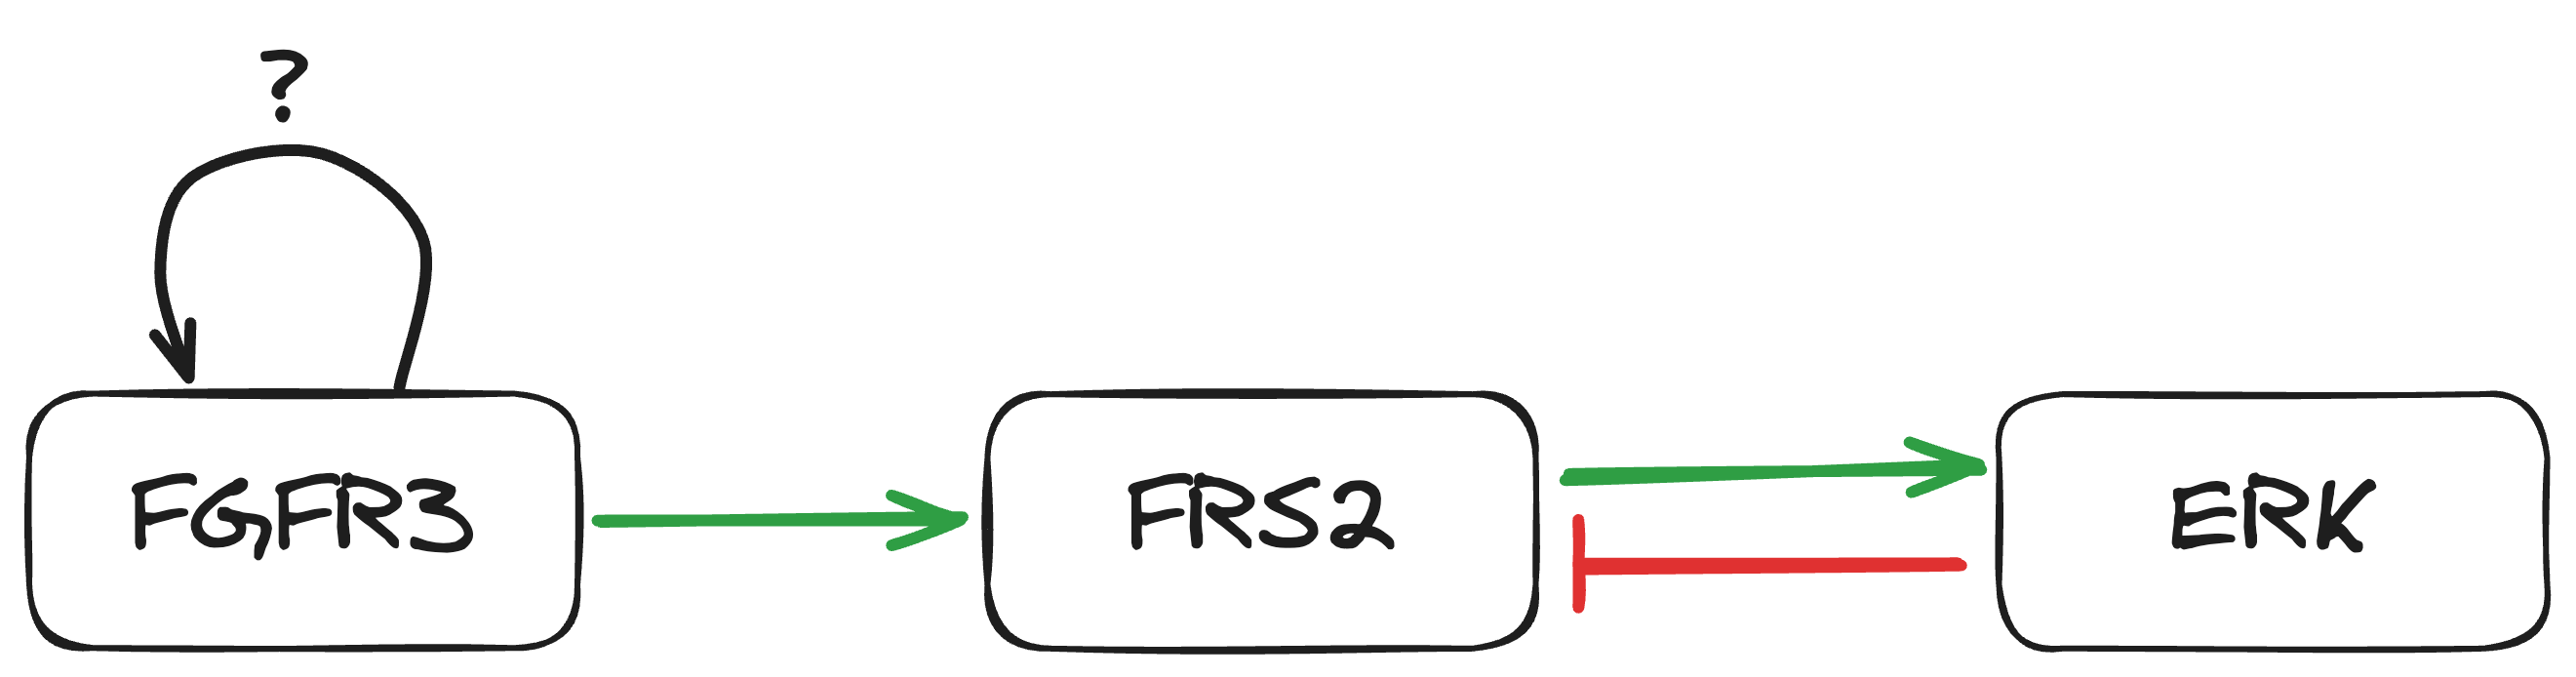
\includegraphics[width=0.6\textwidth]{Figures/regulatory_network.png}
    \caption{\textbf{An example of a simple regulatory network.} The RN contains three nodes and four regulations (two activations, one inhibition and one non-essential self-regulation). The network is a small extract of a MAPK signaling pathway from~\cite{Grieco2013}.} 
    \label{fig:regulatory_network}
    \end{centering}
\end{figure}

\begin{definition}
    Let $\rnMath = (\vertices, \edges)$ denote a directed graph representing the regulatory network, where $\vertices$ is the set of vertices representing the molecular components and $\edges \subseteq \vertices \times \vertices$ is the set of directed edges representing the regulatory interactions between the components.
\end{definition}

% Activations, inhibitions
We call the influence of one substance (regulator) to another (target) a \emph{regulation}. These regulatory effects typically fall into two categories: upregulation (activation), which denotes a positive influence (usually represented in green), or downregulation (inhibition), indicating a negative effect (depicted in red). These types of regulations are \emph{monotonous}; since their impact is consistent. Non-monotonous regulations appear in biological models rarely. When they occur or if the monotonicity is not required, they are depicted in a black color. 

% Observability 
Apart from the monotonicity, another aspect we consider of regulation is \emph{observability}. Observable (essential) regulations were proven by experimentation that the regulator surely influences the target. I.e., in some settings where the regulator is present the regulated substance behaves differently compared to the environment with the lack of the regulator. On the contrary, in case we do not have this certainty, the regulation is \emph{non-essential}. The non-essential regulations should not be over-used. Hypothetically, we could mark all possible RN edges with this type of regulation resulting in a complete, dense graph giving us very little information. Nonetheless, if these regulations occur, they are labelled by a question mark. All other regulations are considered to be observable. We give more formal details about different regulation types in \autoref{ss:bn_definition}.


% RNs are too abstract to be that helpful, we need BN.
Notice, that the influences captured by RNs are highly abstract and that there is very little modeling knowledge present in this model. That is why more specific models are using RNs as a basis. Among these models are ODEs, stochastic gene networks, or Boolean networks, which are described next.


\section{Boolean networks}
\marginpar{
    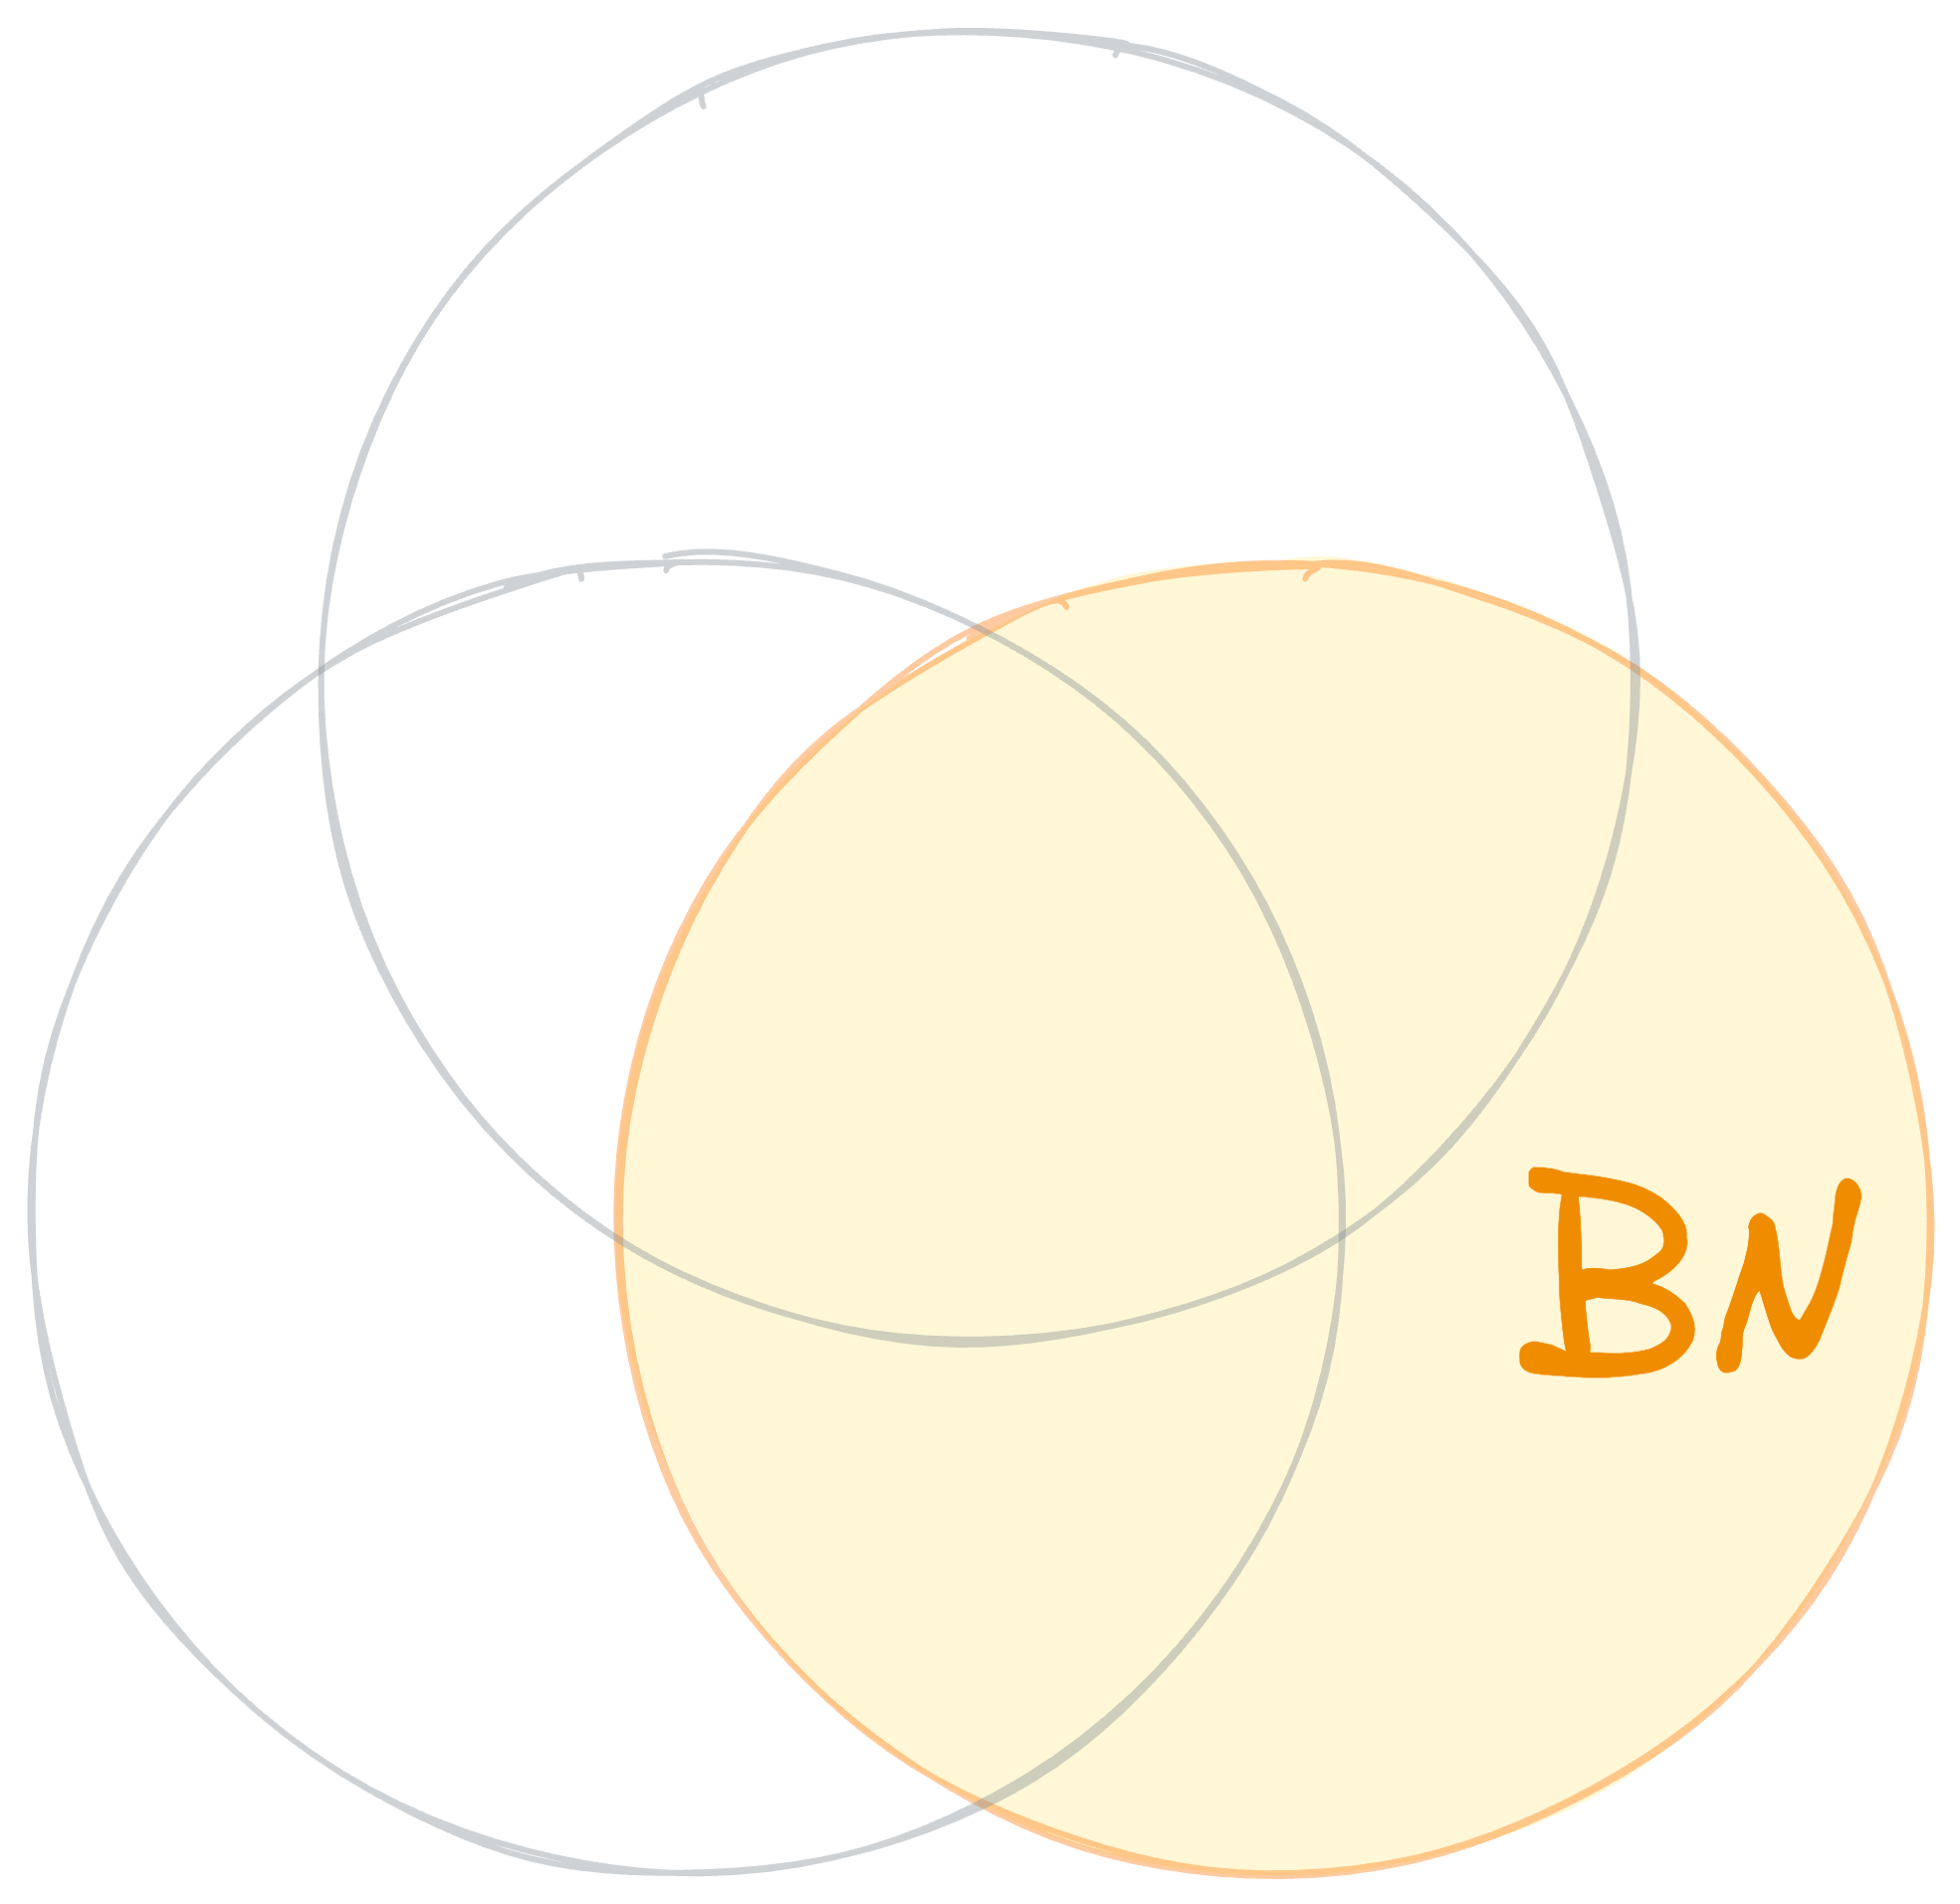
\includegraphics[width=\marginparwidth]{Figures/topics_bns.png}
}
\label{section:boolean-networks}

% Many interactions in biology -> BNs solve this 
The traditional differential equation-based (ODE) models often struggle to capture the intricate interactions and feedback loops present in biological systems due to their complexity. This shortcoming was addressed by Boolean networks (BNs) that were introduced by Kauffman in the 1960s~\cite{Kauffman1969}. Kauffman represented system components as binary variables connected by logical rules. Such an abstraction facilitated the exploration of system dynamics while avoiding the computational complexity of traditional models. 

Since then, it has become a widely used model to study the dynamics of complex biological systems~\cite{Barbuti2020,albert2004}. The Boolean representation also allows researchers to focus on the regulatory relationships and dynamics without getting hindered by detailed biochemical mechanisms. This simplification facilitates efficient analysis of regulatory networks, enabling the discovery of crucial pathways, prediction of system behavior, and identification of pivotal components driving cellular processes.
% Biological systems are characterized by a high amount of interacting elements and their interactions. The Boolean networks (BNs) offer a valuable approach for modeling regulatory networks, providing a way to maintain the structural complexity while ensuring computational feasibility. 

\subsection{Notation}

Here, the notation used in the context of Boolean networks is briefly summarized. For a complete overview of the used notation, refer to \autoref{app:notation}

We consider $0$ and $1$ as interchangeable with $\mathit{false}$ and $\mathit{true}$, respectively. We then define $\bools = \{ 0, 1 \}$ to be the set of Boolean values and $\bools_\unspecified = \{ 0, 1, {\unspecified} \}$ to be an extension of $\bools$ which also admits a \emph{free} value~$\unspecified$ (i.e.~neither $\mathit{true}$ nor $\mathit{false}$). We write $\bools^n$ to denote the set of all $n$-element vectors over $\bools$. For each $x \in \bools^n$, $x_i$ then denotes the $i$-th element of $x$. Finally, for $x \in \bools^n$, index $i \in [1,n]$, and a Boolean value $b \in \bools$, expression $x[i \mapsto b]$ denotes a substitution of the $i$-th element in $x$ for the value~$b$.  Formally, the result is $x' = x[i \mapsto b]$ s.t. $x'_j = b$ for $j = i$, and $x'_j = x_j$ otherwise.

\subsection{Definition}
\label{ss:bn_definition}

We can formally define Boolean networks, as follows:

\begin{definition}
	Let $n$ be the number of system variables. A \emph{Boolean network} is a collection $\bnMath = \{ f_1, \ldots, f_n \}$ with each $f_i: \bools^n \to \bools$ being the Boolean \emph{update function} (sometimes called \emph{local function}) of the network's $i$-th variable.
\end{definition}

A running example of a Boolean network based on the RN from \autoref{fig:regulatory_network} can be seen in \autoref{fig:bn_basic}. Note that, while it is mathematically more convenient to denote variables by their indices, oftentimes we will use their actual names (e.g. $\var{FGFR}$ instead of $f_1$) to present context of the biological system comprehensively.

\begin{figure}[htb]
    \centering
    \subfloat[Regulatory network]{
        \label{subfig:regulatory_network}
        \begin{minipage}[t]{0.35\textwidth}
        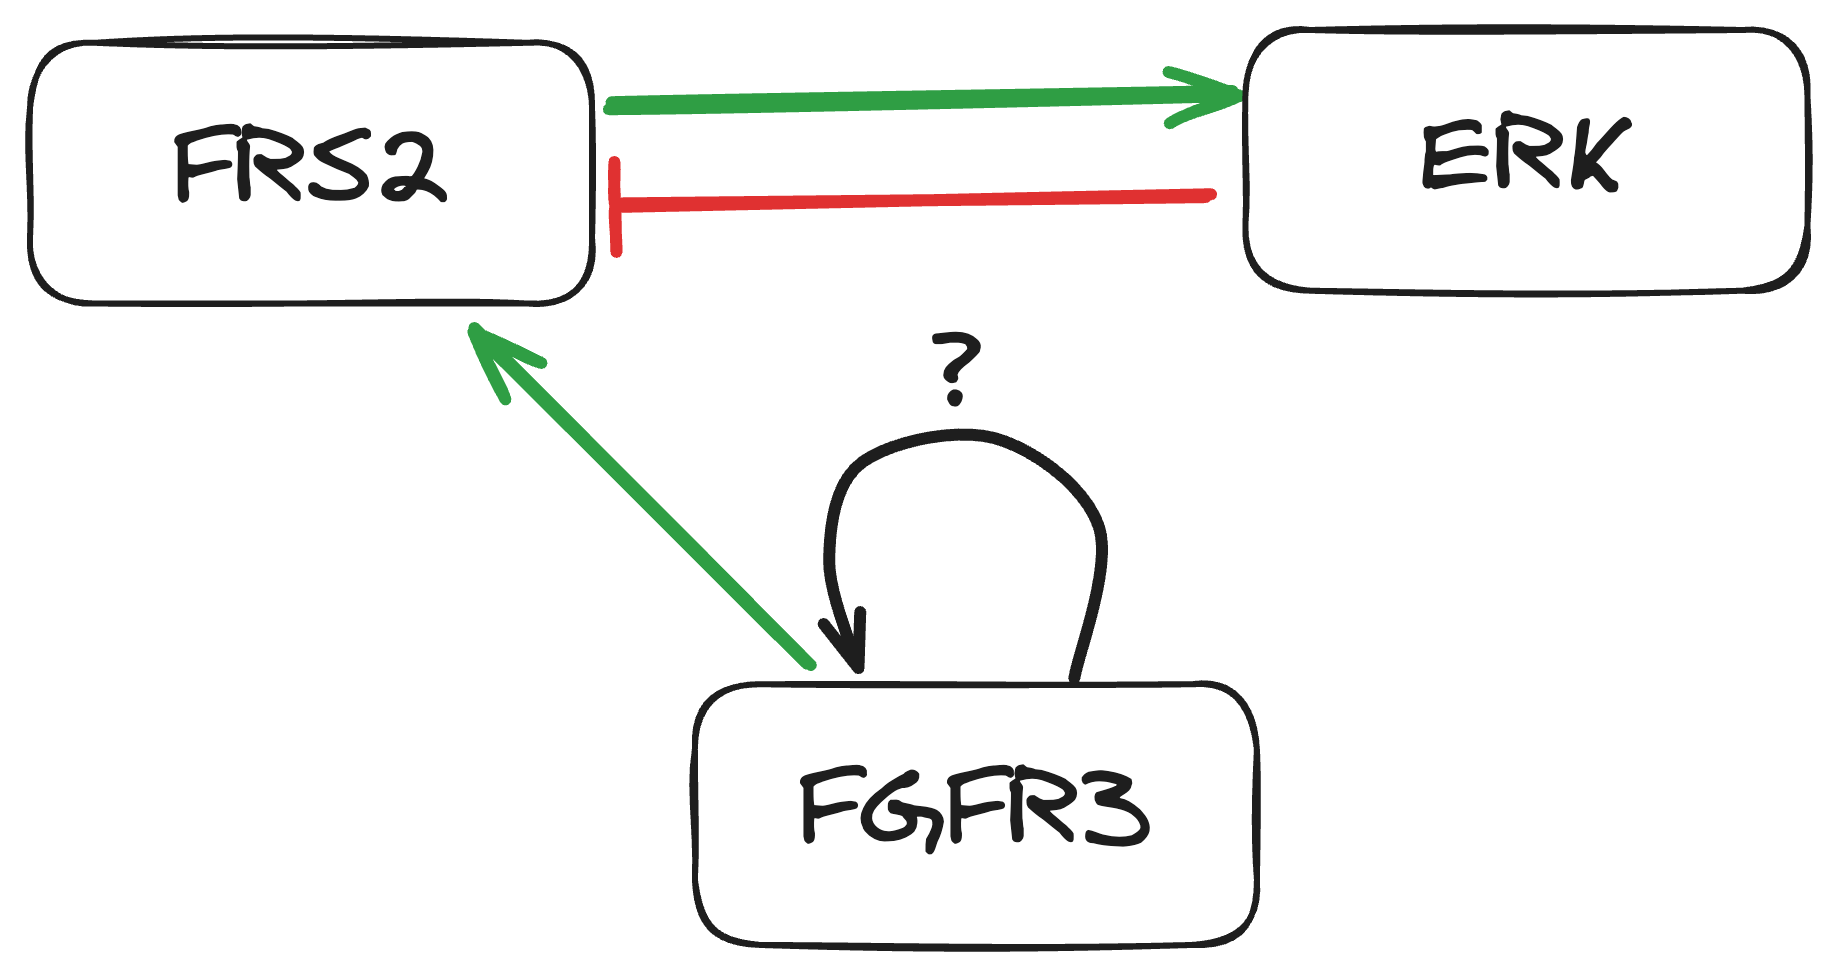
\includegraphics[width=\textwidth,valign=b]{Figures/regulatory_network2.png}
        \end{minipage}
    }
    \subfloat[Boolean network]{
        \label{subfig:bn}
        \begin{minipage}[b]{0.35\textwidth}
        \begin{align*}
            \var{FGFR} &= 1 \\
            \var{FRS2} &= \var{FGFR} \land \neg \var{ERK} \\
            \var{ERK} &= \var{FRS2}
        \end{align*}
        \end{minipage}
    }
    \newline
    \subfloat[State transition graph]{
        \label{subfig:stg}
        \begin{minipage}[t]{0.45\textwidth}
            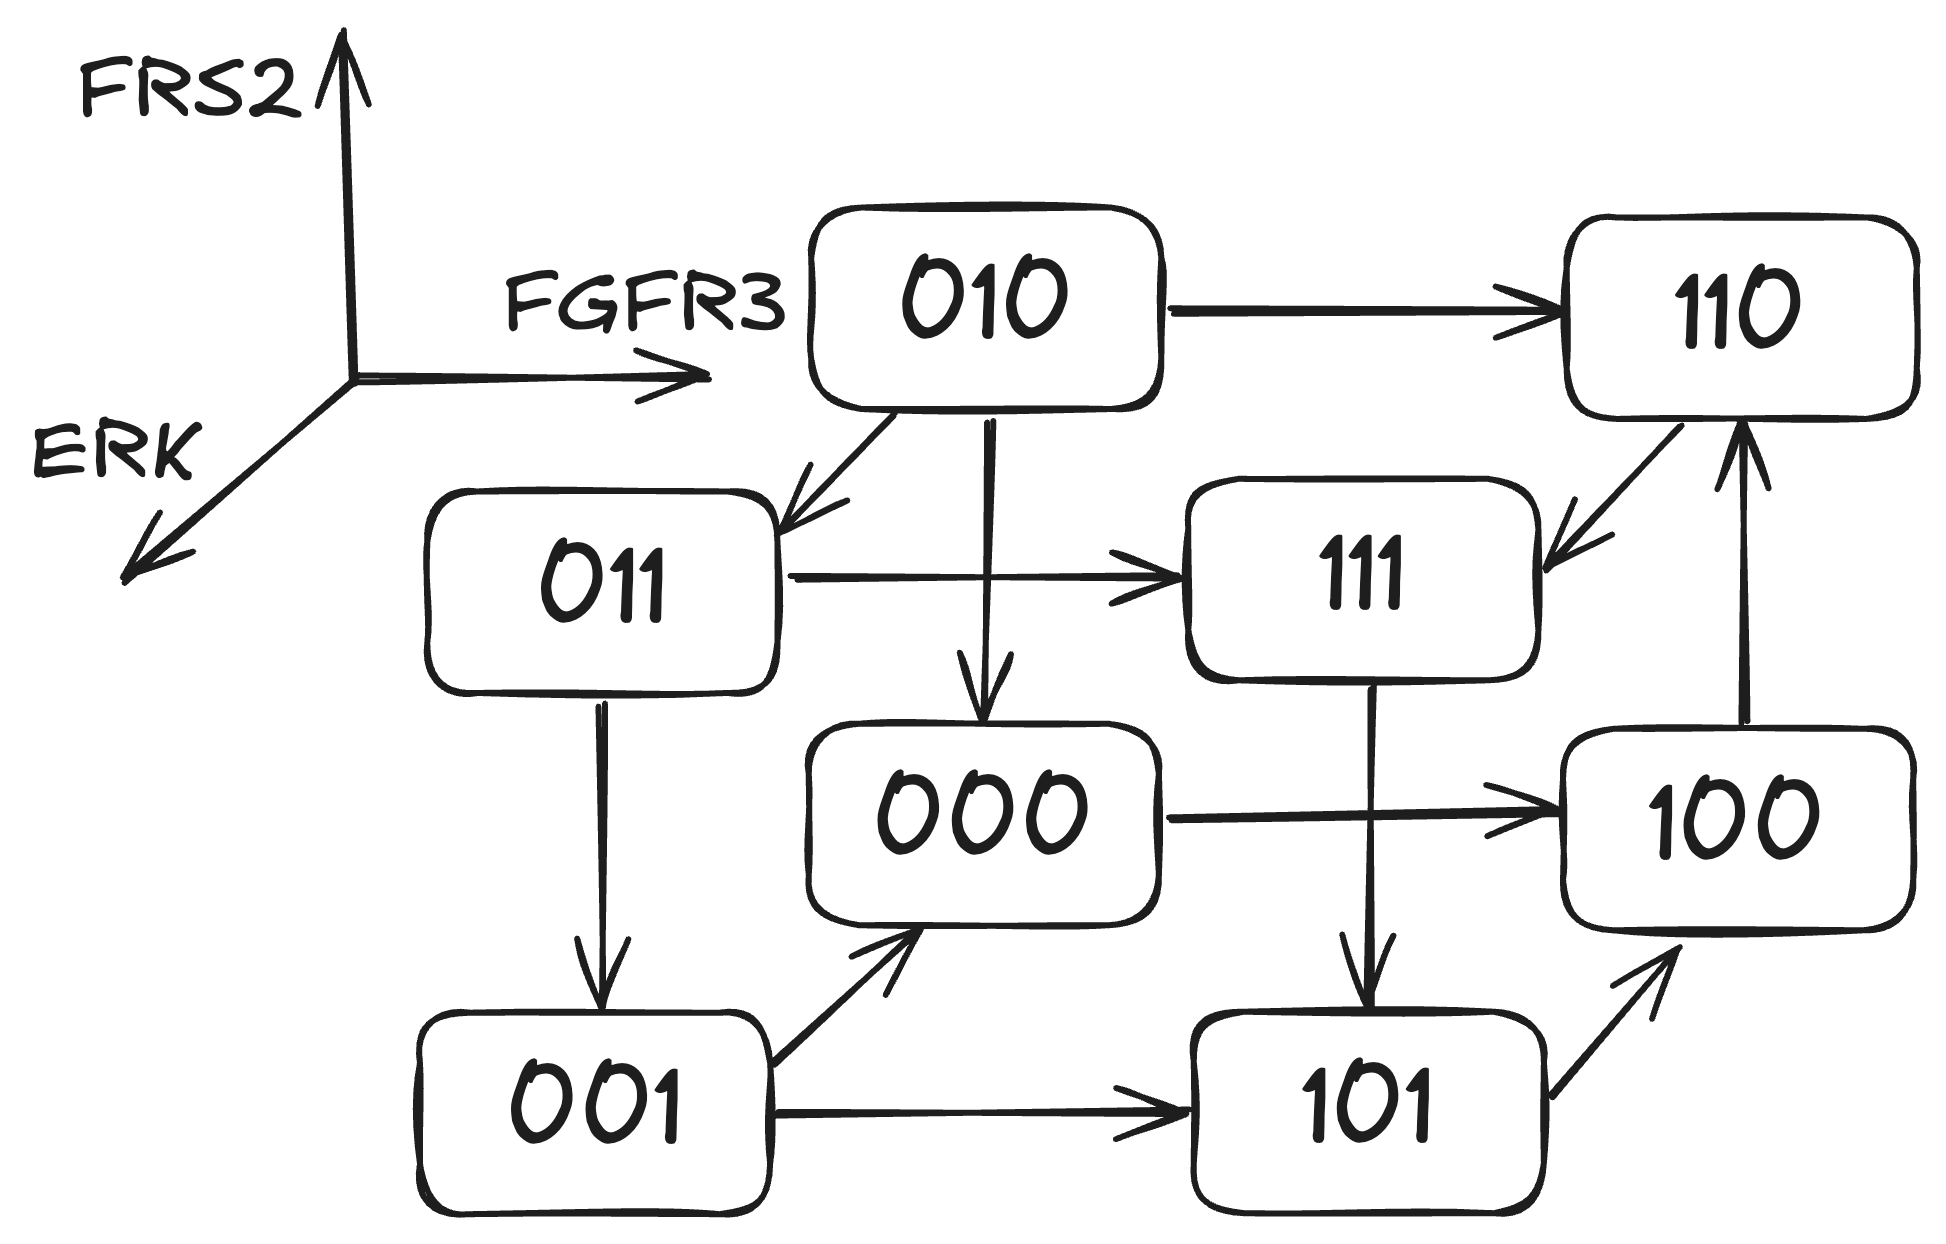
\includegraphics[width=\textwidth,valign=b]{Figures/state_space.png}
        \end{minipage}
    }
    \caption{\textbf{An example of a Boolean network and related concepts.} In \autoref{subfig:regulatory_network}, the same RN as in \autoref{fig:regulatory_network} is displayed for a reader's convenience. This RN is used as a basis for BN defined in \autoref{subfig:bn}. Finally, state-transition graph of the BN is shown in \autoref{subfig:stg} where the labeling of states has the same order as variables order in \autoref{subfig:bn}.} 
    \label{fig:bn_basic}
\end{figure}


% \intention{State space, a state, regulators, inputs, outputs} 
In the context of a specific Boolean network, the set $\bools^n$ is the network's \emph{state space}, and the vectors $x \in \bools^n$ are its \emph{states}. Note that although the input of each $f_i$ is a full state $x \in \bools^n$, the output of $f_i$ does not typically depend on all network variables, but rather on a smaller subset of variables which we say \emph{regulate} the $i$-th variable. These regulations are typically given by a corresponding regulation network. For a BN to respect the regulations defined by its regulation network, the function should comply with the regulation type in following ways:

\begin{itemize}
    \item If a variable $j$ is \emph{essential} for a variable $i$, denoted as $\essential(j,i)$ then: \\ $\exists x \in \bools^n . f_i(x[j \mapsto 1]) \neq f_i(x[j \mapsto 0])$
    \item If variable $j$ \emph{upregulates} (activates) variable $i$, denoted as $\activates(j,i)$: \\
    $ \forall x \in \bools^n . f_i(x[j \mapsto 0]) \Rightarrow f_i(x[j \mapsto 1])$
    \item If variable $j$ \emph{downregulates} (inhibits) variable $i$, or $\inhibits(j,i)$: \\ $\forall x \in \bools^n . f_i(x[j \mapsto 1]) \Rightarrow f_i(x[j \mapsto 0])$
\end{itemize}


If a variable has no regulators (i.e. its update function is a constant), we also call it an \emph{input} of $\bnMath$. Symmetrically, a variable that does not regulate any other variable is called an \emph{output}. For example, when we consider \autoref{subfig:regulatory_network}, if the self-regulation of FGFR3 was not present, FGFR3 would be considered an input.

% Subspaces
Additionally, we call the members of $\bools_\unspecified^n$ the \emph{subspaces} of $\mathbb{BN}$. Intuitively, each subspace $S \in \bools_\unspecified^n$ describes a hypercube in the state space $\bools^n$. This hyper-cube consists of states $x \in \bools^n$ such that $x_i = S_i$ for all $i$ where $S_i \in \bools$. We can thus treat each subspace $S$ as a set of states. Furthermore, to denote a specific subspace, we will often simply use a string of values from $\bools_\unspecified$ instead of the full vector notation (e.g. $S = 11\unspecified0$ instead of $S = (1,1,\unspecified,0)$).	

\subsection{Updating schema}
\label{ss:updating_schemes}

%Briefly discuss synchronous, async and most permisive
In our work, we focus on \emph{asynchronous} semantics for Boolean networks. To give a reader a better overview of the differences between the various semantics, we briefly discuss other common semantics and their trade-offs. A more formal and detailed guide to BN semantics can be found in~\cite{Pauleve2023b}.

In Boolean network modeling, the semantics used to define the update rules of node states significantly influence the system's dynamics and interpretability. \emph{Synchronous} semantics, as introduced in~\cite{Kauffman1969}, operate under the assumption that all nodes in the network update their states simultaneously in discrete time steps. While this approach simplifies analysis and yields deterministic behavior, it imposes an unrealistic constraint on systems such as gene regulatory networks, where simultaneous updating is biologically implausible.

In contrast, \emph{asynchronous} semantics, introduced in~\cite{Thomas1973}, allow for only one node to update at each time step, with a nondeterministic choice of which node updates. This reflects the inherent variability in timing and activity across components in real-world systems, such as the stochastic firing of genes. Asynchronous semantics maintain a more biologically and physically faithful representation of dynamics without the need to introduce explicit timing or probability.

\emph{Probabilistic} semantics introduce randomness directly into the update process. A variable has assigned more than a single update function, while each update function has assigned probability of triggering. This allows the modeling of noise and uncertainty but requires a probabilistic framework and often obscures causal interpretability. 

Lastly, the \emph{most permissive} semantics that was recently introduced in~\cite{Pauleve2020}, define all logically consistent transitions as simultaneously valid, capturing the broadest possible behavior. This is achieved by considering a transient state between 0 and 1 for each variable, allowing any combination of variables to update in a way that is consistent with their logical functions. While useful for exhaustive exploration, this framework might be hard to use for quantification of state-space components since these properties are lost to the abstraction via transient states.

Asynchronous semantics offer a compelling middle ground. They provide a natural and realistic modeling framework for systems where the order and timing of updates are nondeterministic. Nonetheless, they preserve the causal structure of networks and allow for quantifiable tractable analysis while avoiding the oversimplification of synchronous updates.

% STG
To formally reason about the evolution of the network's state, we consider asynchronous state-transition graph of BNs:

\begin{definition}
	Given a Boolean network $\mathbb{\bnMath} = \{ f_1, \ldots, f_n \}$, the \emph{state-transition graph} $\STG(\bnMath) = (\vertices, \edges)$ is a directed graph with $\vertices = \bools^n$ and $\edges \subseteq \vertices \times \vertices$ given as follows:
	$$
		(u,v) \in \edges \Leftrightarrow (u \not= v \land \exists i \in [1,n].~v = u[i \mapsto f_i(u)])
	$$
\end{definition}

The \emph{state-transition graph} $\STG(\bnMath)$ captures the dynamics of the Boolean network by representing its states and transitions. An example is graphically depicted in \autoref{subfig:stg}.

% \intention{Maximal fair runs} 
The behavior of a network is then studied through its \emph{maximal strongly fair runs}. Here, a maximal run $\run: \NatsZero \to \bools^n$ represents an infinite sequence of states where for every $t \in \NatsZero$, we have either $\run(t) = \run(t+1)$, or $\run(t) \to \run(t+1)$. That is, the state either remains constant, or updates according to $\STG(\bnMath)$. 

Furthermore, we are only concerned with \emph{strongly fair} runs~\cite{Abadi1995,Mandon2019CMSB}. These are runs which do not delay any available transition indefinitely. Formally, let $\run$ be a run and $x \in \bools^n$ a state that appears infinitely often in $\run$, such that $x \to y$ for some $y \in \bools^n$. Then $\run$ is fair only if $y$ also appears infinitely often in $\run$ as a successor to $x$. To denote the set of such states that appear infinitely often in a run $\run$, we write $inf(\run) = \{ x \in \bools^n \mid \forall k \in \NatsZero, \exists t > k.~\run(t) = x \}$. Finally, we may write $x \in \run$ as a shorthand for $\exists t.~\run(t) = x$ and a set of all possible runs in $\bnMath$ is denoted as $\allRuns(\bnMath)$.

\subsection{State space structures}
\label{ss:state_space_structures}

% \intention{Bridge to state space structures} 
The focus on strongly fair runs naturally leads to the notions of trap set, trap space, and attractor, which dictate the long-term behavior of the corresponding BN:

\begin{definition}
	Let $\bnMath = \{ f_1, \ldots, f_n \}$ be a Boolean network and $X \subseteq \bools^n$ a set of network states. We say that $X$ is a \emph{trap set} when for all $x \in X$ and $y \in \bools^n$ we have that $x \to y$ implies $y \in X$ (i.e., $X$ cannot be escaped). A subspace $X = \bools^n_\unspecified$ which is also a trap set can be also called a \emph{trap space}. The $X$ is an \emph{attractor} when $X$ is strongly connected within $\STG(\bnMath)$.
\end{definition}

\begin{figure}[bth]
    \centering
    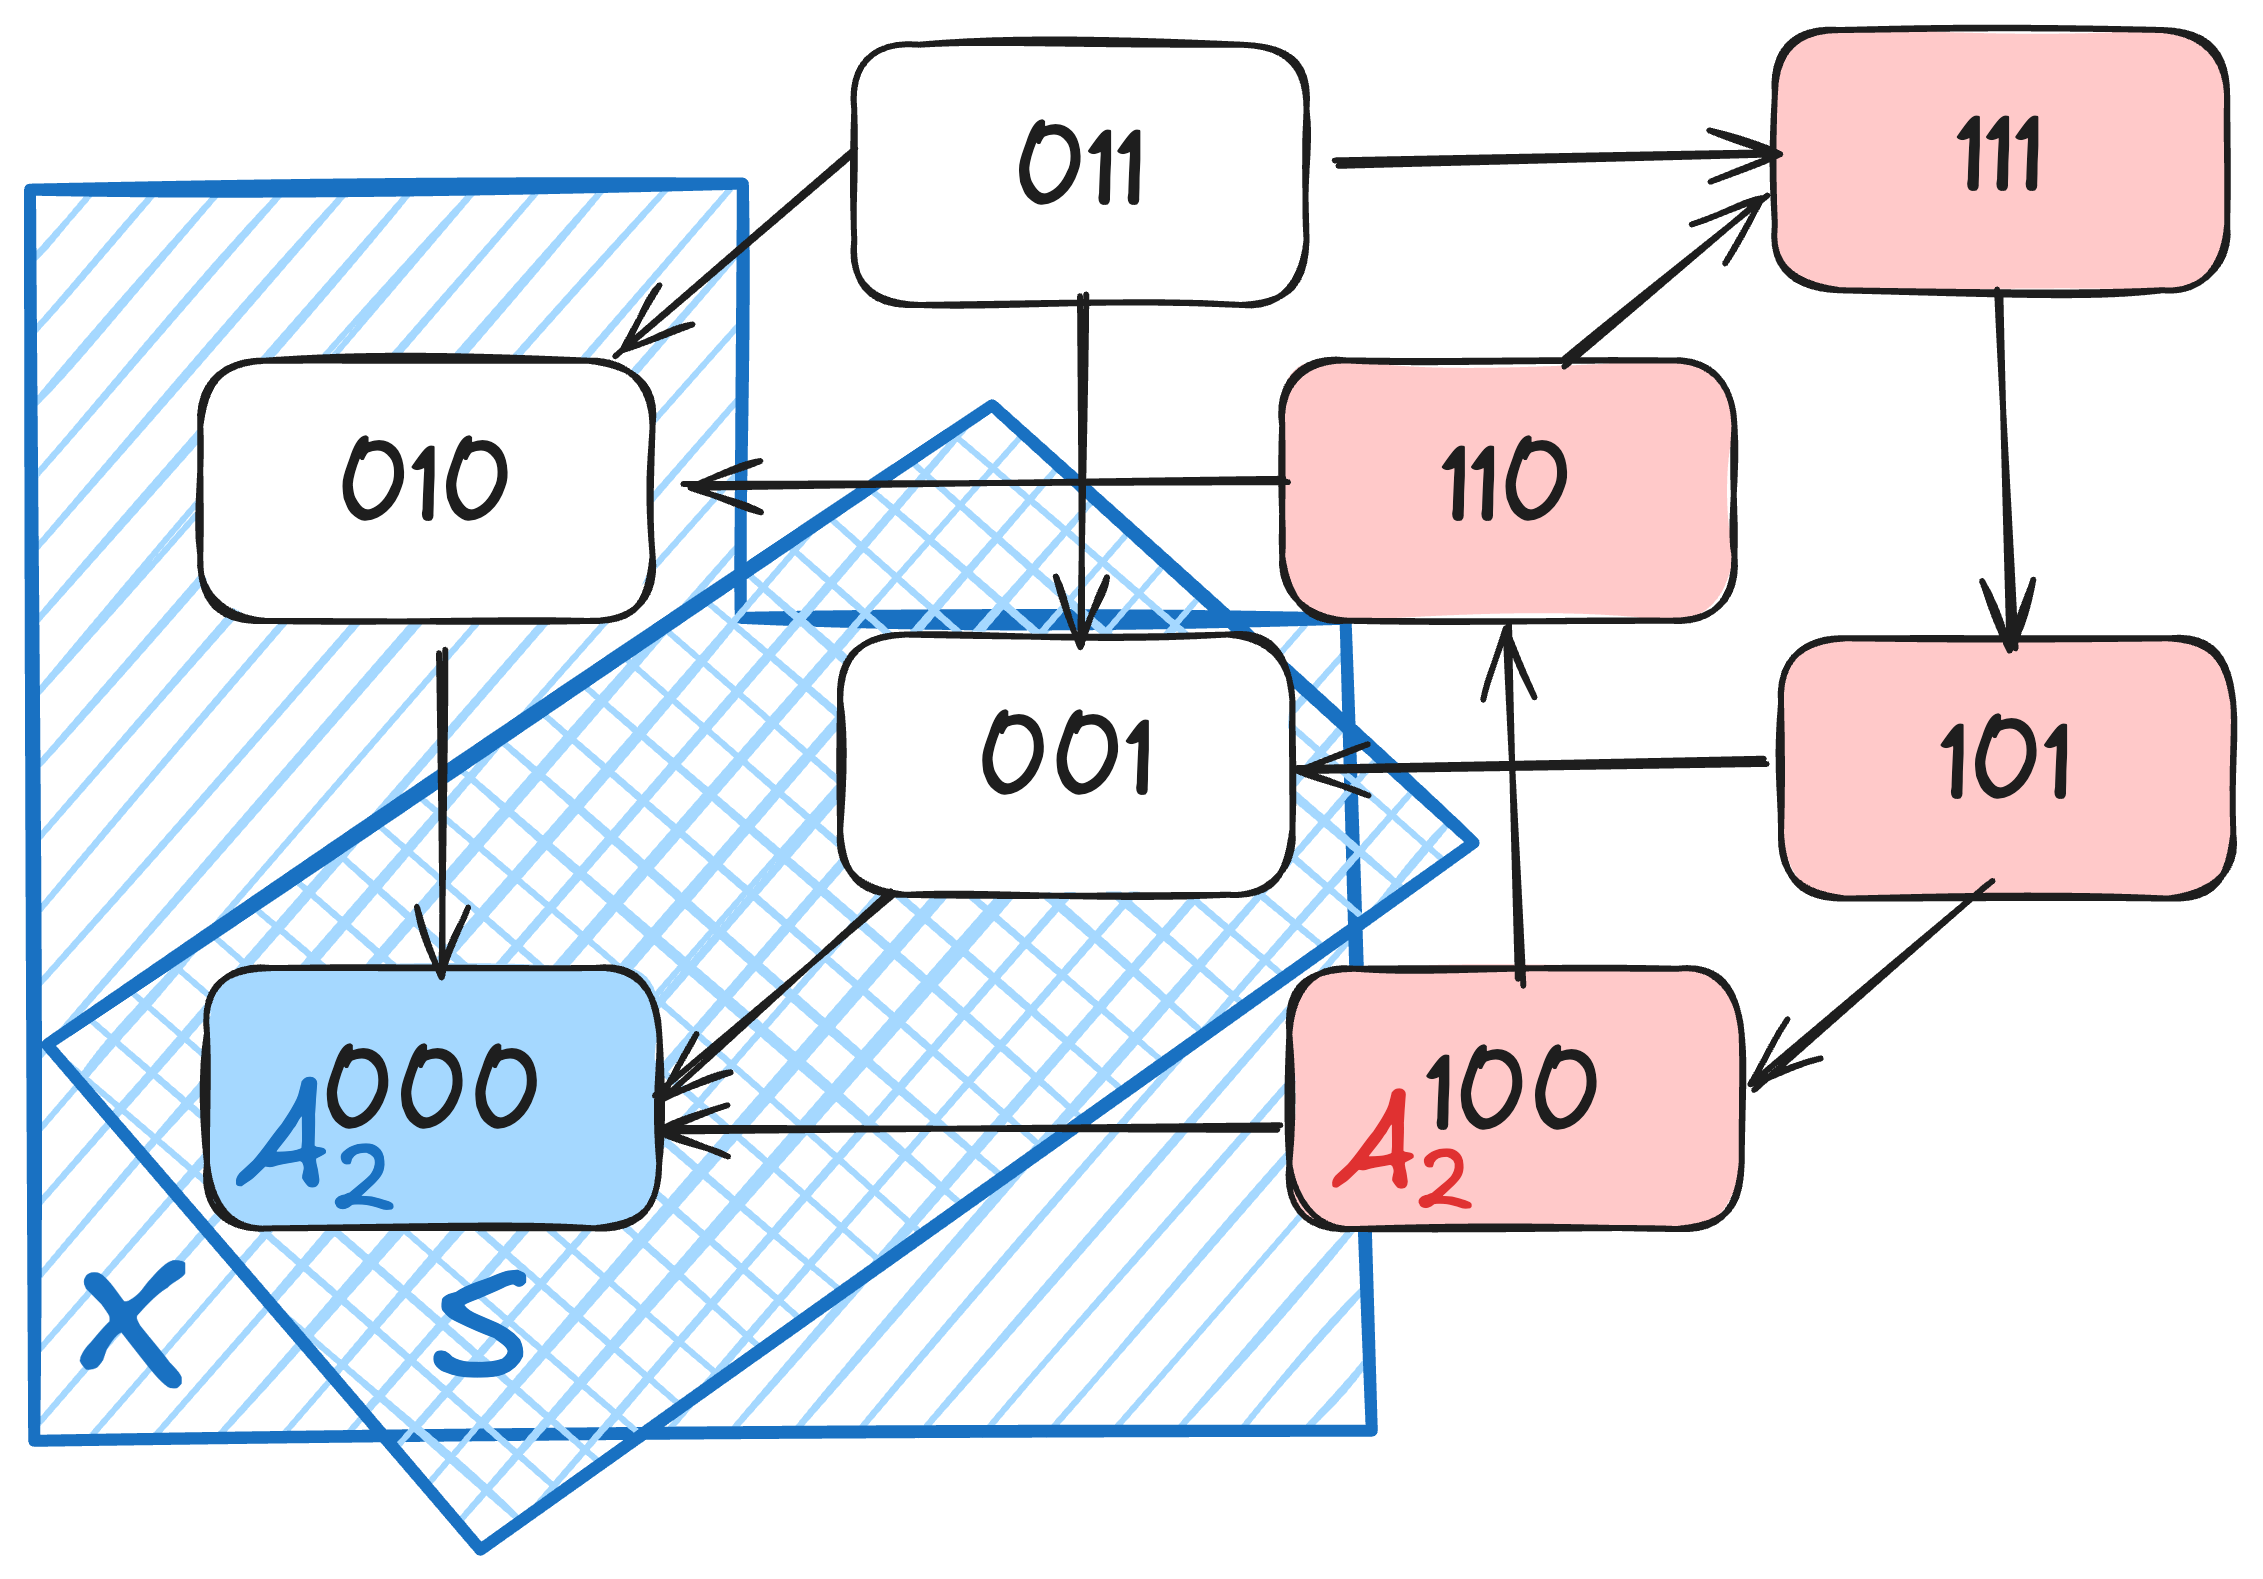
\includegraphics[width=0.4\textwidth]{Figures/traps.png}
    \caption{
        \textbf{Difference between a trap set and a trap space.} A state space of a BN with $n=3$ is shown. The BN contains two attractors: a steady state $A_1$ (a blue state 000) and an oscillatory attractor $A_2$ (red states $1\unspecified\unspecified$). The trap set $S$ (double-shaded are) is also a trap space as it can be described by a subspace $00\unspecified$. On the other hand, the trap set $X$ (shaded area) is not a trap space as it cannot be described by a subspace. Notice, that also a set of all states $\unspecified\unspecified\unspecified$ is a trap space (set), even though it contains multiple attractors.
    }
    \label{fig:traps}
\end{figure}

% \intention{Attractors} 
For a visualization of the concepts, see \autoref{fig:traps}. Equivalently, we can define an attractor $A$ as the inclusion-minimal trap set of $\bnMath$. 

Notice, that an attractor of a run is exactly the set of states that appear infinitely often in the run $inf(\run) = A$. We write $\allAttractors(\STG(\bnMath))$ to denote the set of all attractors of $\bnMath$. An attractor containing only a single state is called a \emph{steady state} or \emph{fixed point}. On the other hand, we will refer to attractors containing multiple states as \emph{oscillatory attractors}*. \marginpar{*Some works also distinguish oscillatory (where period of states repeating in the sequence is strictly regular) and chaotic attractors~\cite{Pastva2022}. In this work we call both these types as oscillatory.}

Finally, observe that due to our fairness assumption, all runs admitted by $\STG(\bnMath)$ eventually reach some attractor. As such, for each strongly fair $\pi$, the set of states that appear infinitely often in $\pi$ is always an attractor. For example, if we consider the BN from \autoref{fig:bn_basic}, it has a single attractor; the oscillation in subspace $0\unspecified\unspecified$. All runs of this BN eventually reach this attractor.

% \textcolor{red}{Basins, weak basin, strong basin}
Given an attractor, we also define its \emph{basin of attraction} as the set of all states that can reach the attractor. The larger the basin of attraction, the attractor is more likely to be biologically relevant~\cite{Klemm2005}. Due to the non-deterministic nature of asynchronous BNs, individual states may reach multiple attractors depending on the selected successor states. To that end, we recognize two types of basins of attraction~\cite{Klarner2018,Schwab2020}:

\begin{definition}
    \label{def:basins}
    The \emph{weak basin of attraction} comprises all states which can lead to the given attractor: 
    $$\weakBasin{\bnMath, \attractor} = \{ x \in \bools^n \mid \exists \run \in \allRuns(\bnMath): x \in \run \land (\forall s \in \attractor : s \in \run) \}$$

    In contrast, the \emph{strong basin of attraction} includes all states from which the given attractor is eventually surely reached.
    $$\strongBasin{\bnMath, \attractor} = \{ x \in \bools^n \mid \forall \run \in \allRuns(\bnMath): x \in \run \Rightarrow (\forall s \in \attractor : s \in \run) \}$$
\end{definition}

If Boolean network $\bnMath$ is clear from the context, it can be omitted from the notation. States which belong to a strong basin of attraction lead to only one possible attractor. In contrast, states in the weak basin of attractor may lead to a certain attractor but also another one. This concept is also shown in \autoref{fig:basins}. As we will see later in \autoref{chapter:source_target_control}, these notions are particularly useful in the context of BN control.

\begin{figure}[bth]
    \centering
    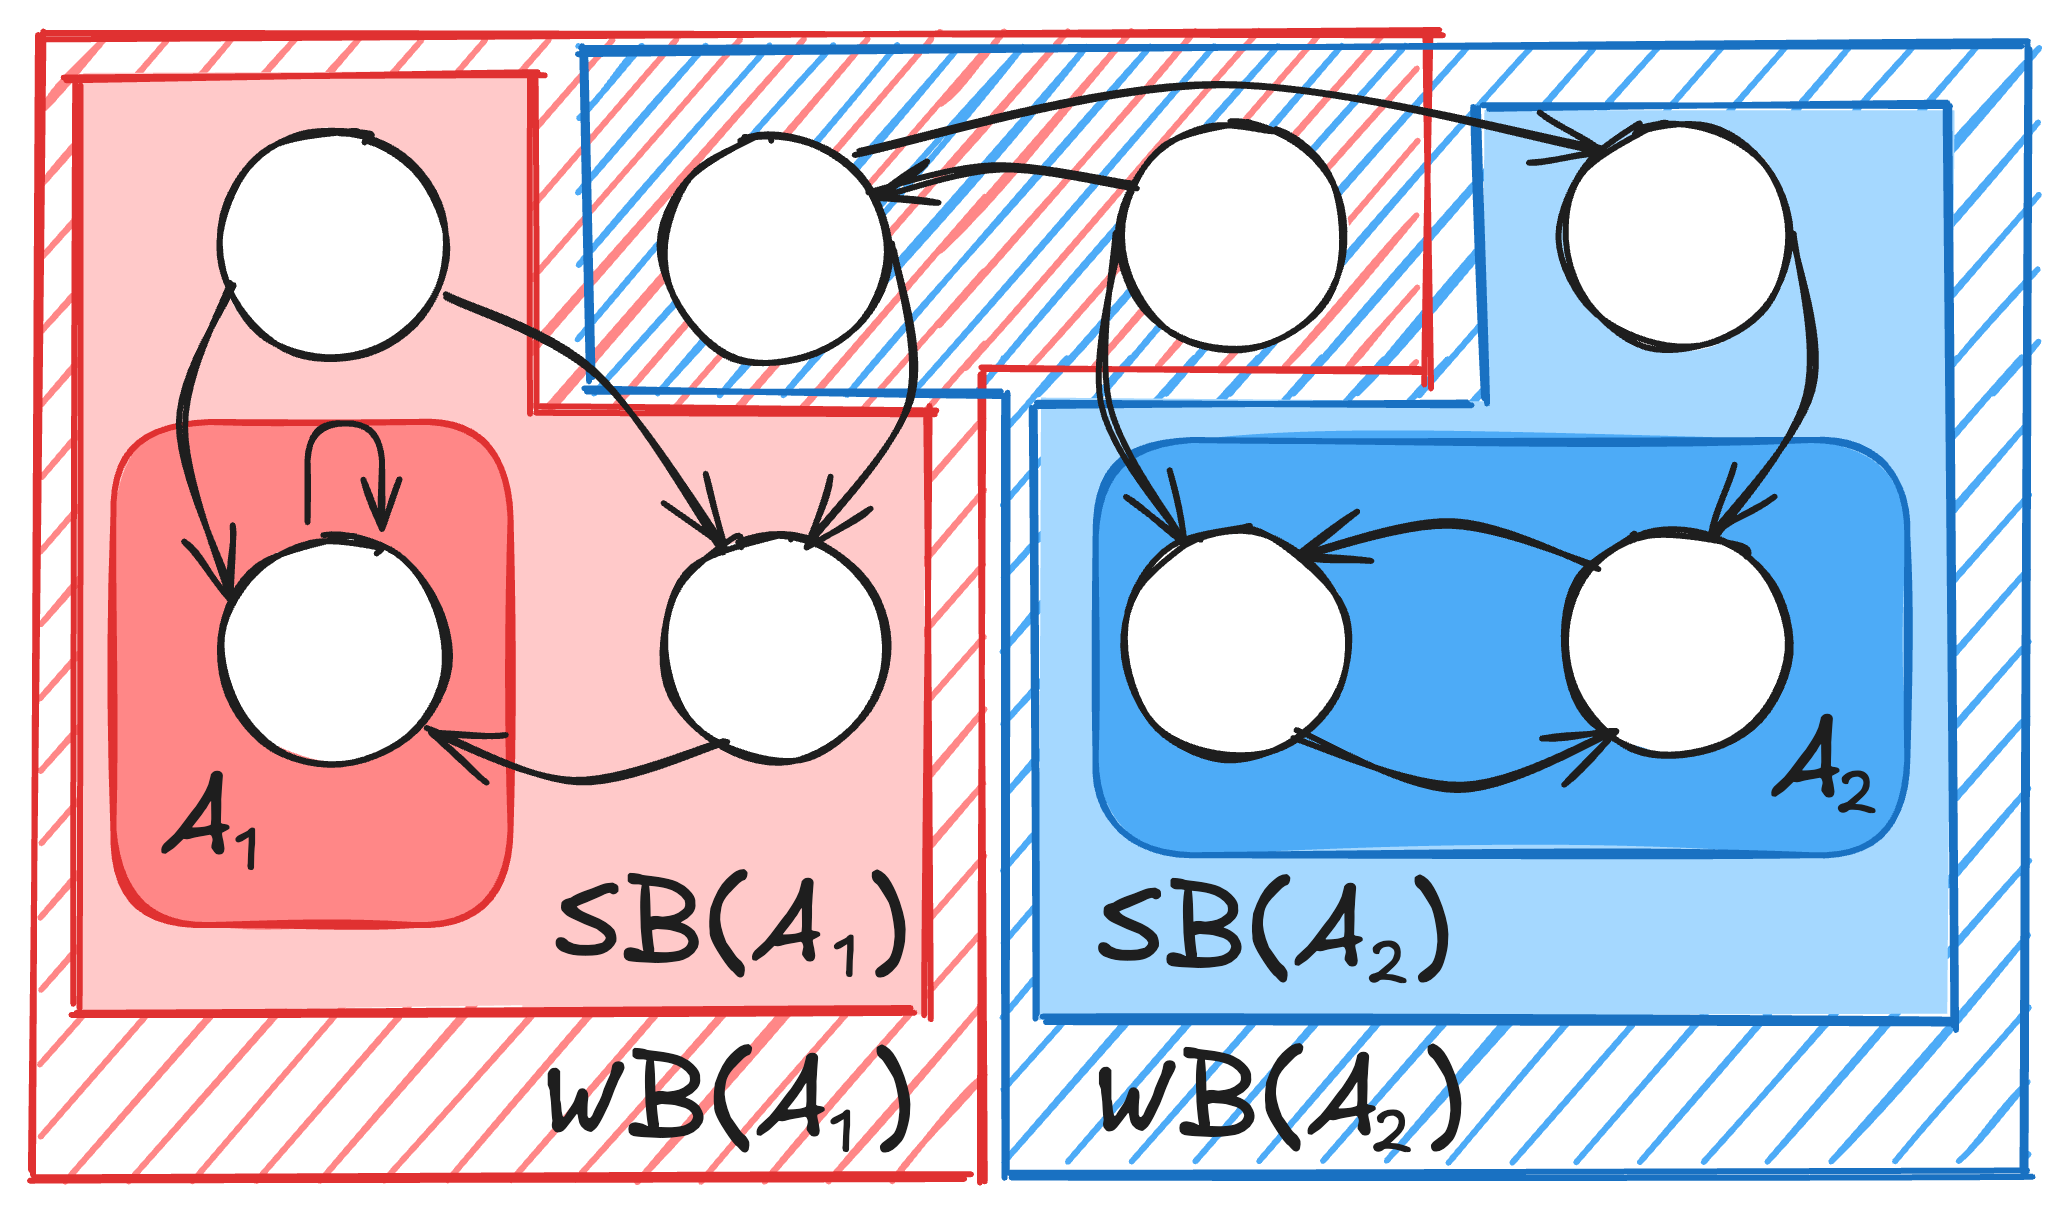
\includegraphics[width=0.8\textwidth]{Figures/basins.png}
    \caption{
        \textbf{Difference between a strong and a weak basin.} The figure shows a simple STG with two attractors: a steady state $A_1$ (dark red) and an oscillatory attractor $A_2$ (dark blue). Strong basins of $A_1$ and $A_2$ are shown in light red and light blue, respectively and are disjoint. Finally, the weak basin of $A_1$ and $A_2$ are shown in red and blue stripes, respectively. The weak basins overlap as some states can reach multiple attractors.
    }
    \label{fig:basins}
\end{figure}

\subsection{Summary}

In this section, we summarized the key concepts related to Boolean networks and their dynamics. We introduced the notions of states and updating schemas. We have introduced state space structures, such as trap sets and attractors, which are crucial for understanding the long-term behavior of Boolean networks Building on these concepts, we now turn our attention to the control of Boolean networks.

\section{Control of Boolean networks}
\label{s:control_of_bns}
\marginpar{
    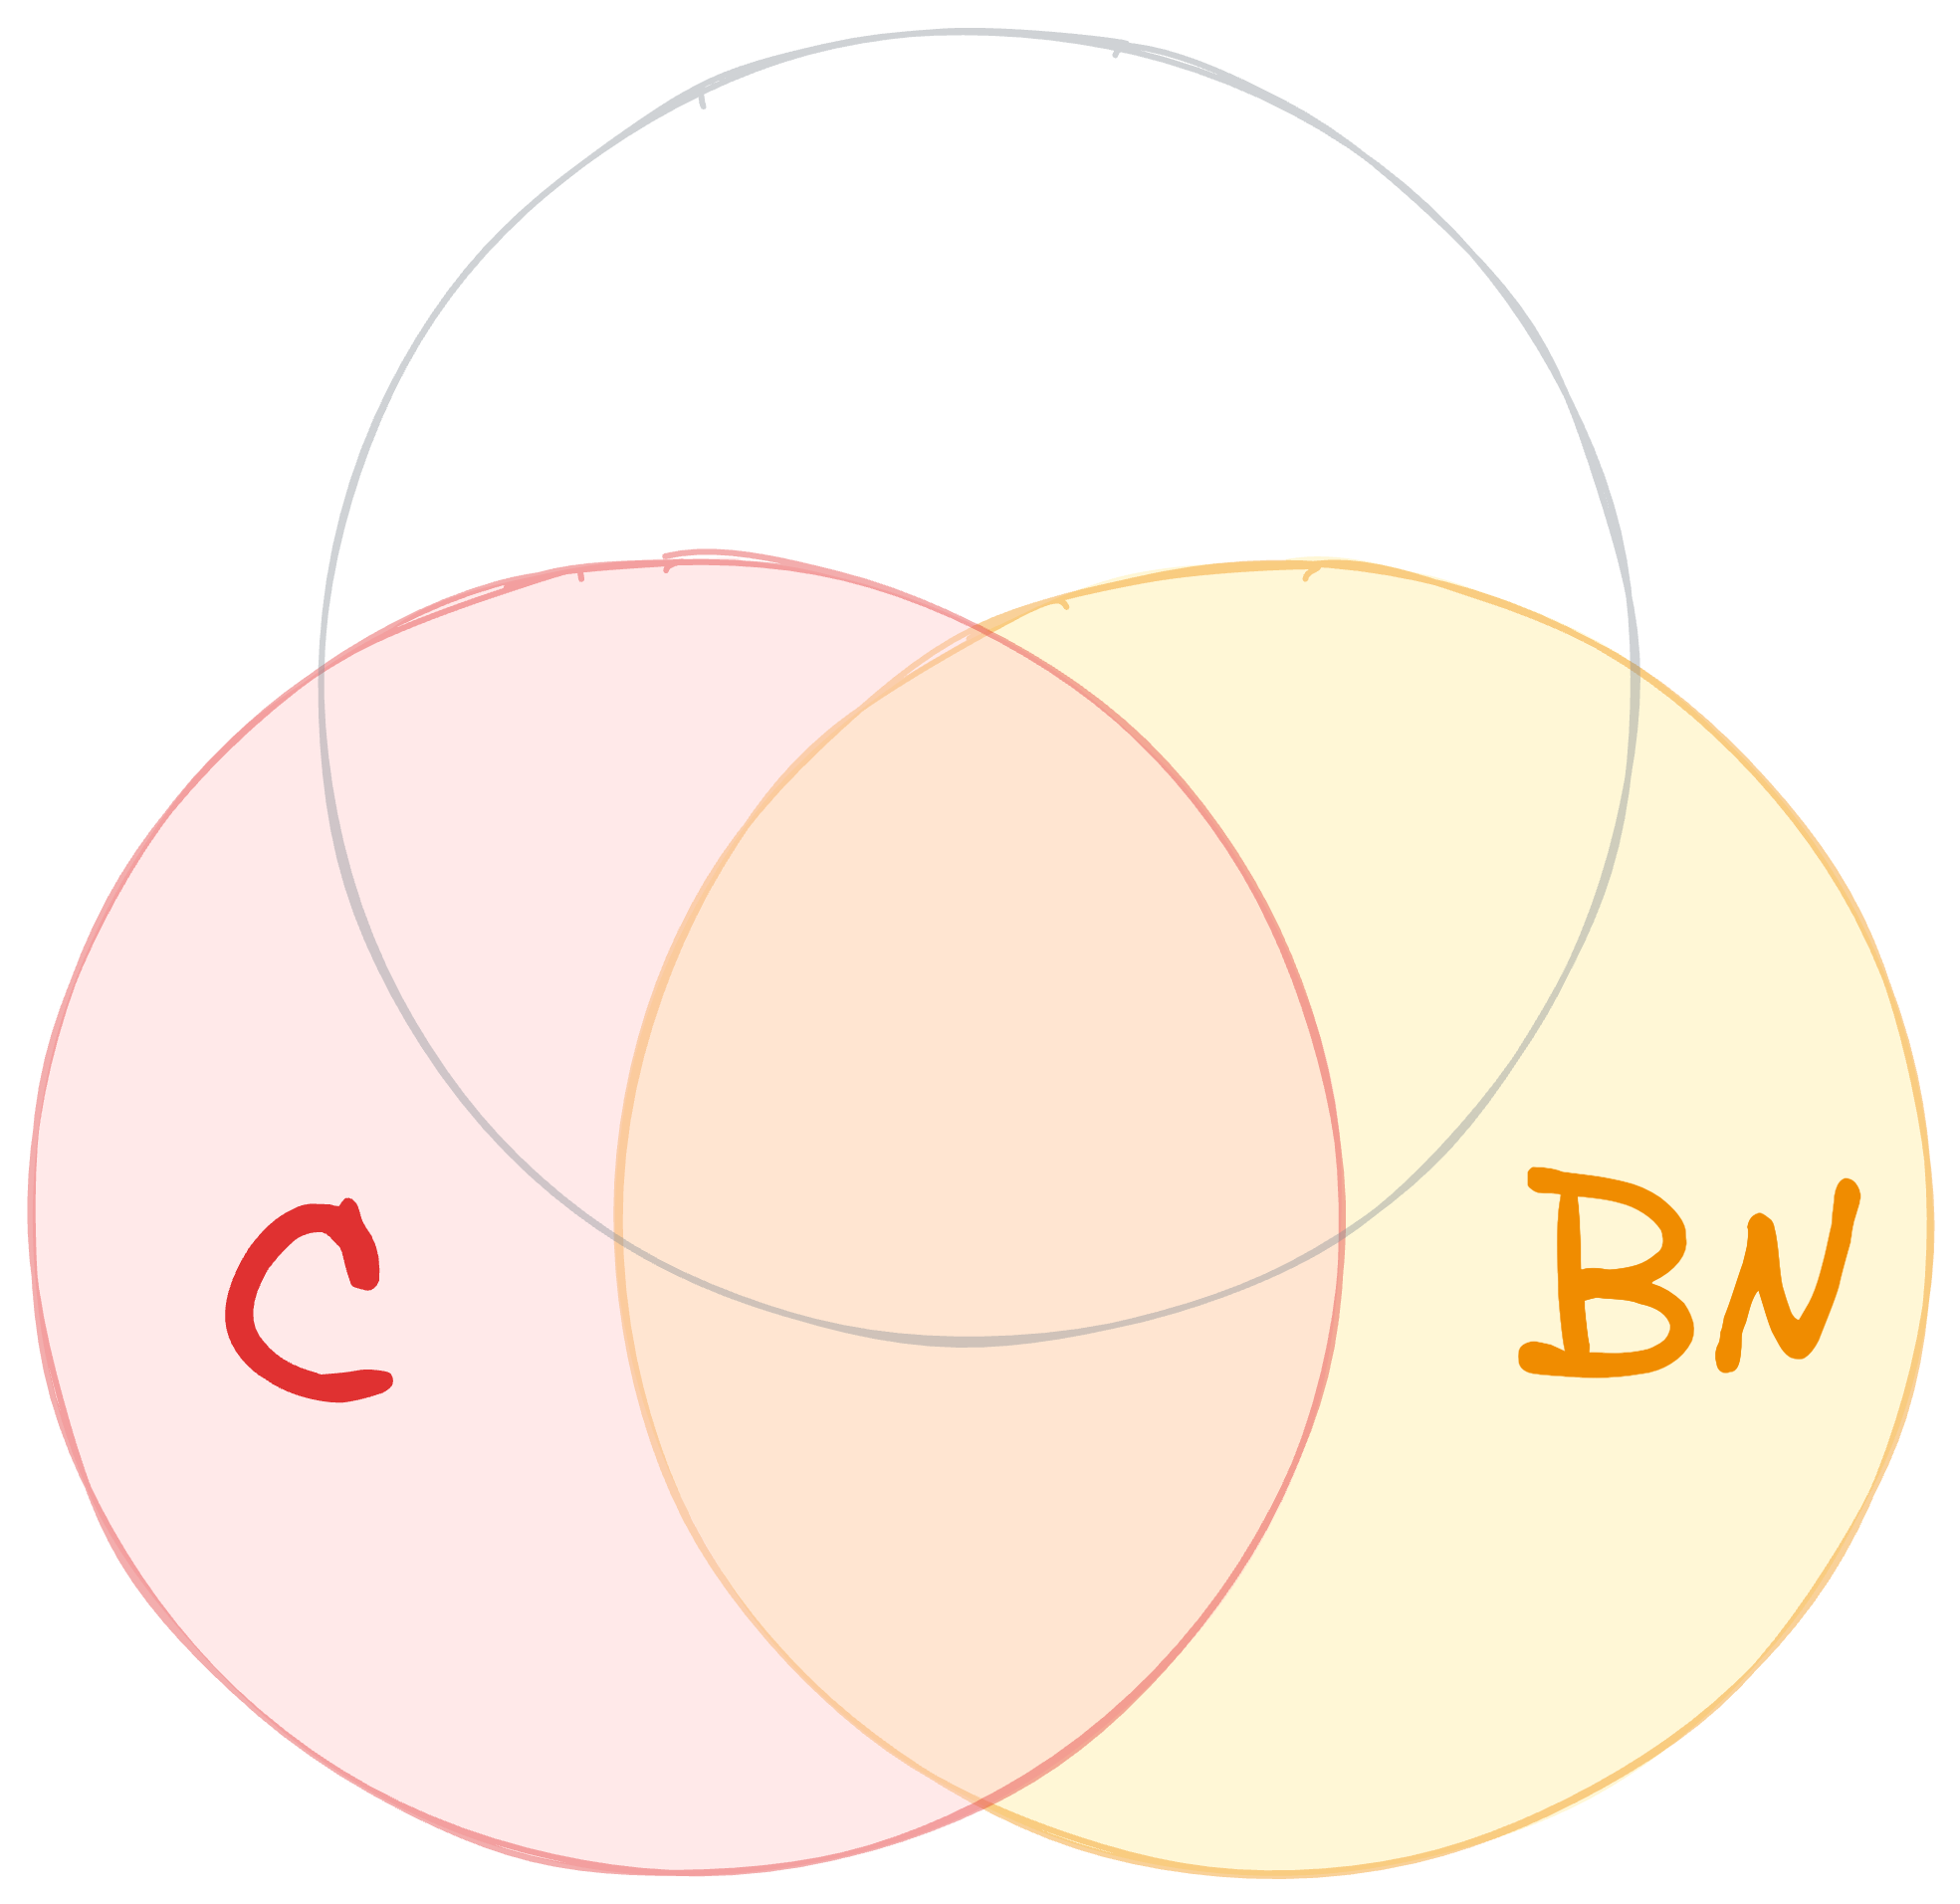
\includegraphics[width=\marginparwidth]{Figures/topics_ctrl_bn.png}
}


In this section we zoom into the \emph{control} of Boolean networks. We first discuss different control objectives that have been studied in the literature. Then, we introduce the concept of perturbations, which are the means of controlling a Boolean network. Finally, we summarize the aspects in which the problem of control of Boolean networks differ.

\subsection{Control objective} \label{sss:controlObj}

% Source-target, target, full control, all pair
The first aspect in which control problems differ is ``what kind of stabilization we are trying to achieve''. Since the only component stable in a BN are its attractors, the control objectives typically focus on navigating a system to reach a certain attractor or a set of attractors.

There are two base types of control objectives: \emph{existential} and \emph{inevitable} control~\cite{Paul2018SETTA,Mandon2019PHD}. Existential control aims to find a strategy that make for a system \emph{possible} to reach the target. On the other hand, universal control seeks a strategy that \emph{ensures} convergence to the target attractor from any initial state. In this work, we consider only the inevitable control objectives.

We consider five different control objectives based on the previous lines of research~\cite{Baudin2019,Fontanals2020}. The differences between control objectives are also illustrated in \autoref{fig:st}:

\begin{enumerate}
\item \emph{Source-target control}: Given a \emph{source state} $s \in \bools^n$, and a \emph{target attractor} $T \in \allAttractors$, ensure, that the BN converges from the state $s$ to the attractor $T$ (see \autoref{subfig:st_a}).
\item \emph{Target control}: Given a \emph{target attractor} $T \in \allAttractors$, ensure that for \emph{any} initial state $s \in \bools^n$ the BN converges from $s$ to $T$ (see \autoref{subfig:st_b}).
\item \emph{Full control}: Find a set of control strategies such that for all pairs of distinct attractors $S, T \in \allAttractors$, applying a strategy from this set guarantees that the BN converges from $S$ to $T$ (see \autoref{subfig:st_c}).
\item \emph{All-pairs control}: Given a subset of source attractors $\mathcal{S} \subseteq \allAttractors$ and target attractors $\mathcal{T} \subseteq \allAttractors$, find a set of perturbations such that for every pair $S \in \mathcal{S}$ and $T \in \mathcal{T}$, applying a subset of the perturbations guarantees that the BN converges from $S$ to $T$ (similar to full control in~\autoref{subfig:st_c}).
\item \emph{Phenotype control}: Given a subset of states $X \subseteq \bools^n$, ensure that from any initial state, the BN converges to an attractor $A \subseteq \allAttractors$ such that $A \subseteq X$ (\autoref{subfig:st_d}).
\end{enumerate}


\begin{figure}[htb]
    \centering
    \subfloat[Source-target control]{
        \label{subfig:st_a}
        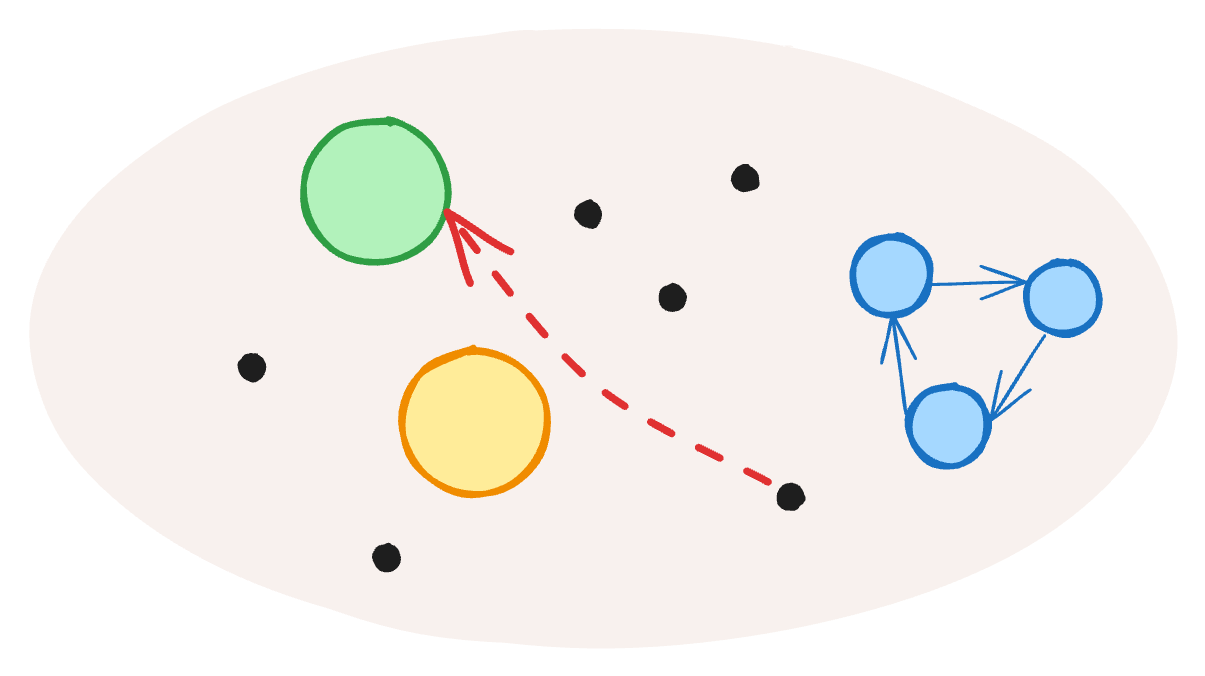
\includegraphics[width=0.4\textwidth,valign=b]{Figures/st_a.png}
    }
    \subfloat[Target control]{
        \label{subfig:st_b}
        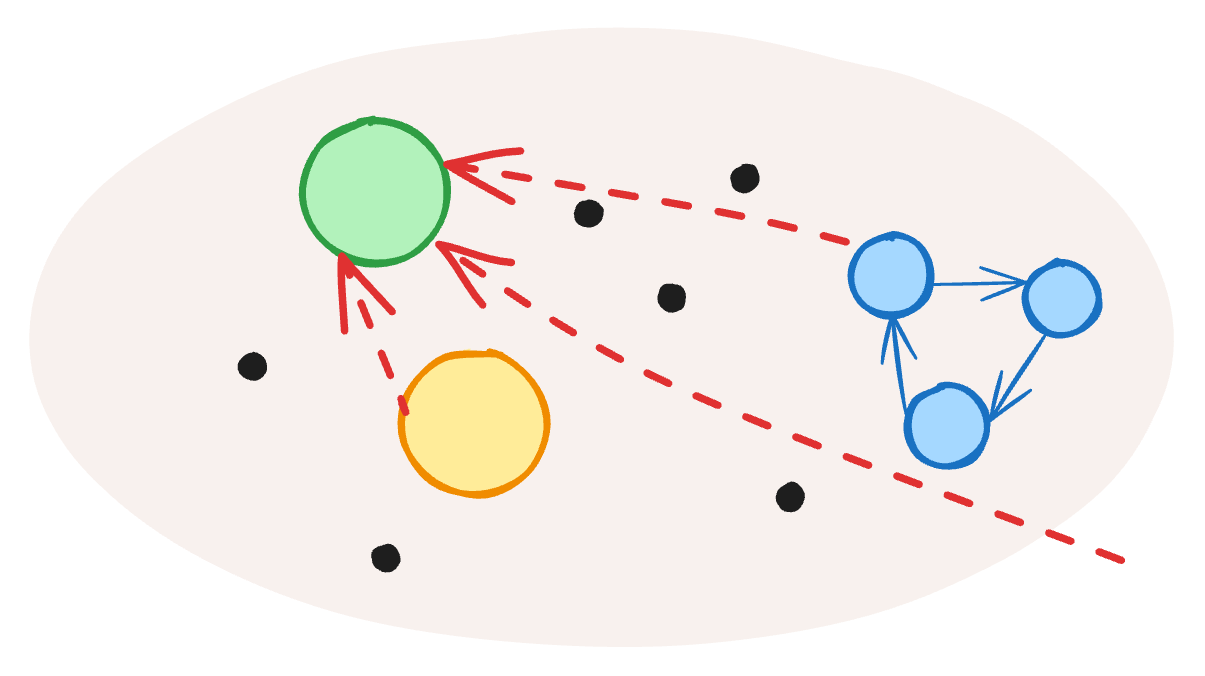
\includegraphics[width=0.4\textwidth,valign=b]{Figures/st_b.png}
    }
    \newline
    \subfloat[Full control]{
        \label{subfig:st_c}
        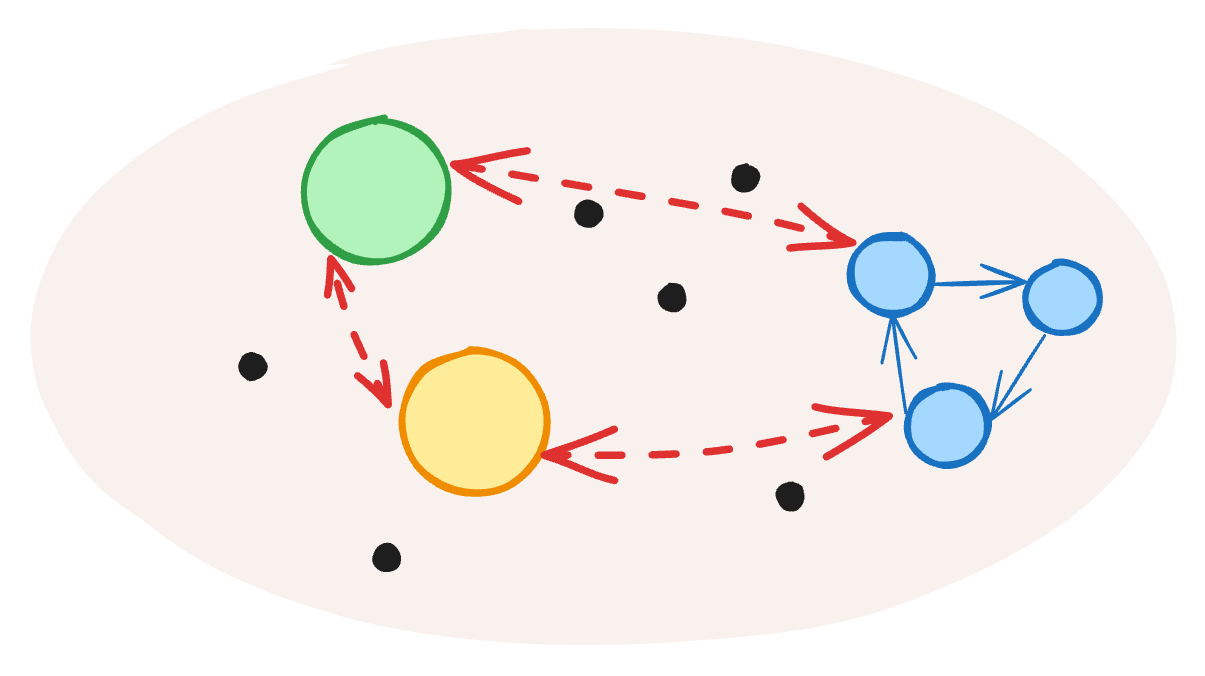
\includegraphics[width=0.4\textwidth,valign=b]{Figures/st_c.png}
    }
    \subfloat[Phenotype control]{
        \label{subfig:st_d}
        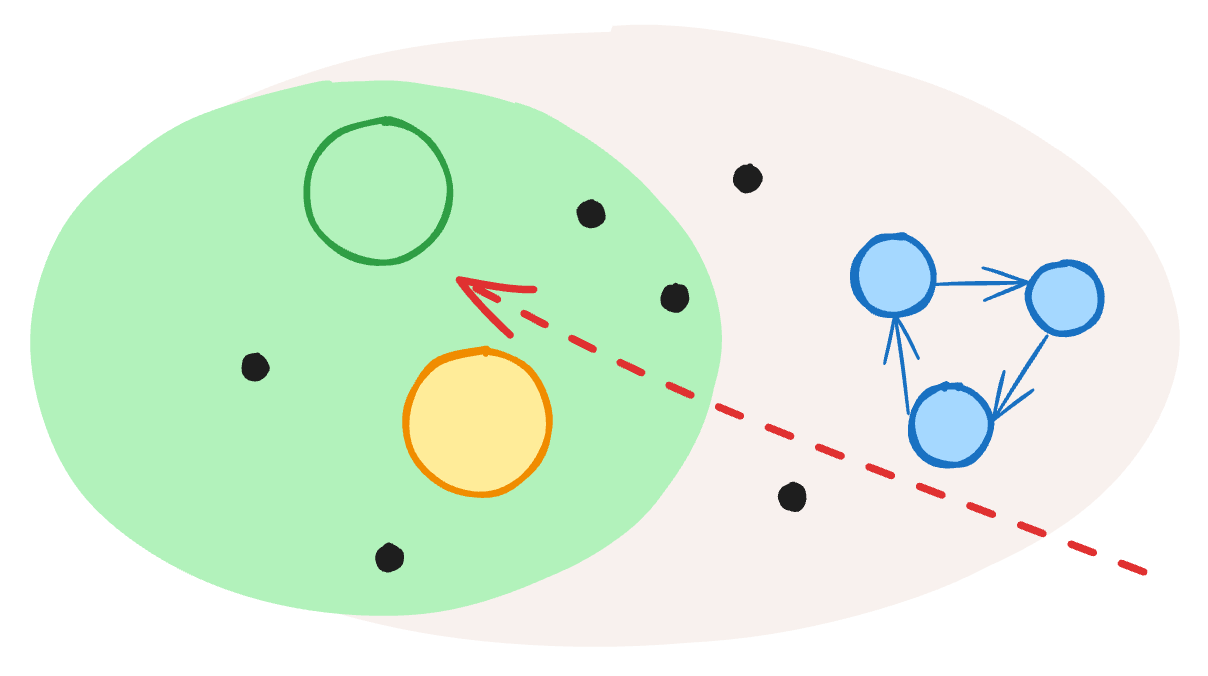
\includegraphics[width=0.4\textwidth,valign=b]{Figures/st_d.png}
    }
    \caption{\textbf{Difference between control objectives.} The black points are non-attractor states of BN, the colorful points are attractors, and the red arrows shows where we are trying to stabilize by applying the control. The green area in the \autoref{subfig:st_d} represents a target phenotype.} 
    \label{fig:st}
\end{figure}


The control objectives as defined above are rather high-level since they do not specify using what means are allowed to achieve the goals. In particular, they do not clarify what types of perturbations can be applied to the system in order to guide it towards the desired attractors. Therefore, we discuss the perturbations next.

\subsection{Perturbations}
\label{subsec:perturbations}
% Explain perturbations and their types
\emph{Perturbations} are the means of controlling a Boolean network. In order to ensure that a network always reaches some attractor which it does not reach in some of its normal runs, logically, we need to interfere with the system in some way. This is exactly what perturbations are -- a forced intervention to the dynamics of a system. There are several types of perturbations, but in this work we focus on \emph{variable perturbations}, which override the value of some variables in the network by constant values. 

Other types of perturbations are \emph{function perturbations} which can override the update functions completely and in a more complex way. However, due to their complexity, they were so far considered only within a context of synchronous Boolean networks~\cite{Liu2017, Xiao2007}. Somewhat less abstract is a concept of \emph{edge perturbations} which can disable or enable certain regulations in the network~\cite{Fontanals2022c}. Both these two notions can be considered within the framework of partially specified Boolean networks, however due to their complexity both in regard to formalization and practical application, they were not included in this work, and we leave their exploration for future research.

The perturbations are formally defined as follows:

\begin{definition}
\label{def:perturbation}
Given a Boolean network $\bnMath = \{f_1, \dots, f_n \}$, a \emph{variable perturbation} is a vector $\perturbation \in \bools_\unspecified^n$. For every $\perturbation_i = \unspecified$, we say that the $i$-th variable is \emph{unperturbed}, whereas for $\perturbation_i = 0$ or $\perturbation_i = 1$, we say that the variable is \emph{perturbed} (to either $0$ or $1$). The \emph{size} of $\perturbation$ is the number of perturbed variables: $\size(\perturbation) = \; \mid \{ i \mid \perturbation_i \neq \unspecified \} \mid$. A perturbation can again be seen as a \emph{subspace} of the $\bnMath$ state space $\bools^n$. The set of all considered perturbations is denoted as $\allPerturbations$ and typically equals to $\bools_\unspecified^n$. 
\end{definition}

We further recognize two special types of perturbations based on their size; an \emph{empty perturbation} is a perturbation of size $0$ (i.e., $\perturbation = \unspecified\unspecified\ldots\unspecified$) which does not perturb any variable, for short, denoted as \emptyPerturbation. In contrast, a \emph{trivial perturbation} is a perturbation of size $n$ (i.e., $\perturbation \in \bools^n$) which perturbs all variables in the network to a value of the target state. Finally, if a perturbation is very small (i.e one or two being perturbed), we can denote it as an assignment of perturbed variables instead of a full vector. For example, for $n=4$, instead of writing $\perturbation = 1\unspecified0\unspecified$, we can write $\{ \var{v1}=1, \var{v3}=0 \}$.

Usually, the perturbations are expensive. Therefore, we want to keep the amount of performed perturbations as small as possible. Thus, control is an optimization problem and is typically measured by a perturbation size (number of perturbed variables), but other criteria might be considered as well.

It can be seen, that the definition of perturbation is rather abstract and does not specify how the perturbation is applied. To make perturbations applicable, we need to consider also \emph{temporal} properties of perturbations.

\subsection{Temporal properties of perturbations}
% \intention{Single-step, temporary, permanent perturbations} 
The perturbations differ based on their temporal characteristics. The first classification is based on the length of the applied perturbation. We consider \emph{one-step}, \emph{temporary}, and \emph{permanent} perturbations. \autoref{fig:otpc} shows an intuition on the differences between these types of perturbations. 

\begin{figure}[bth]
    \centering
    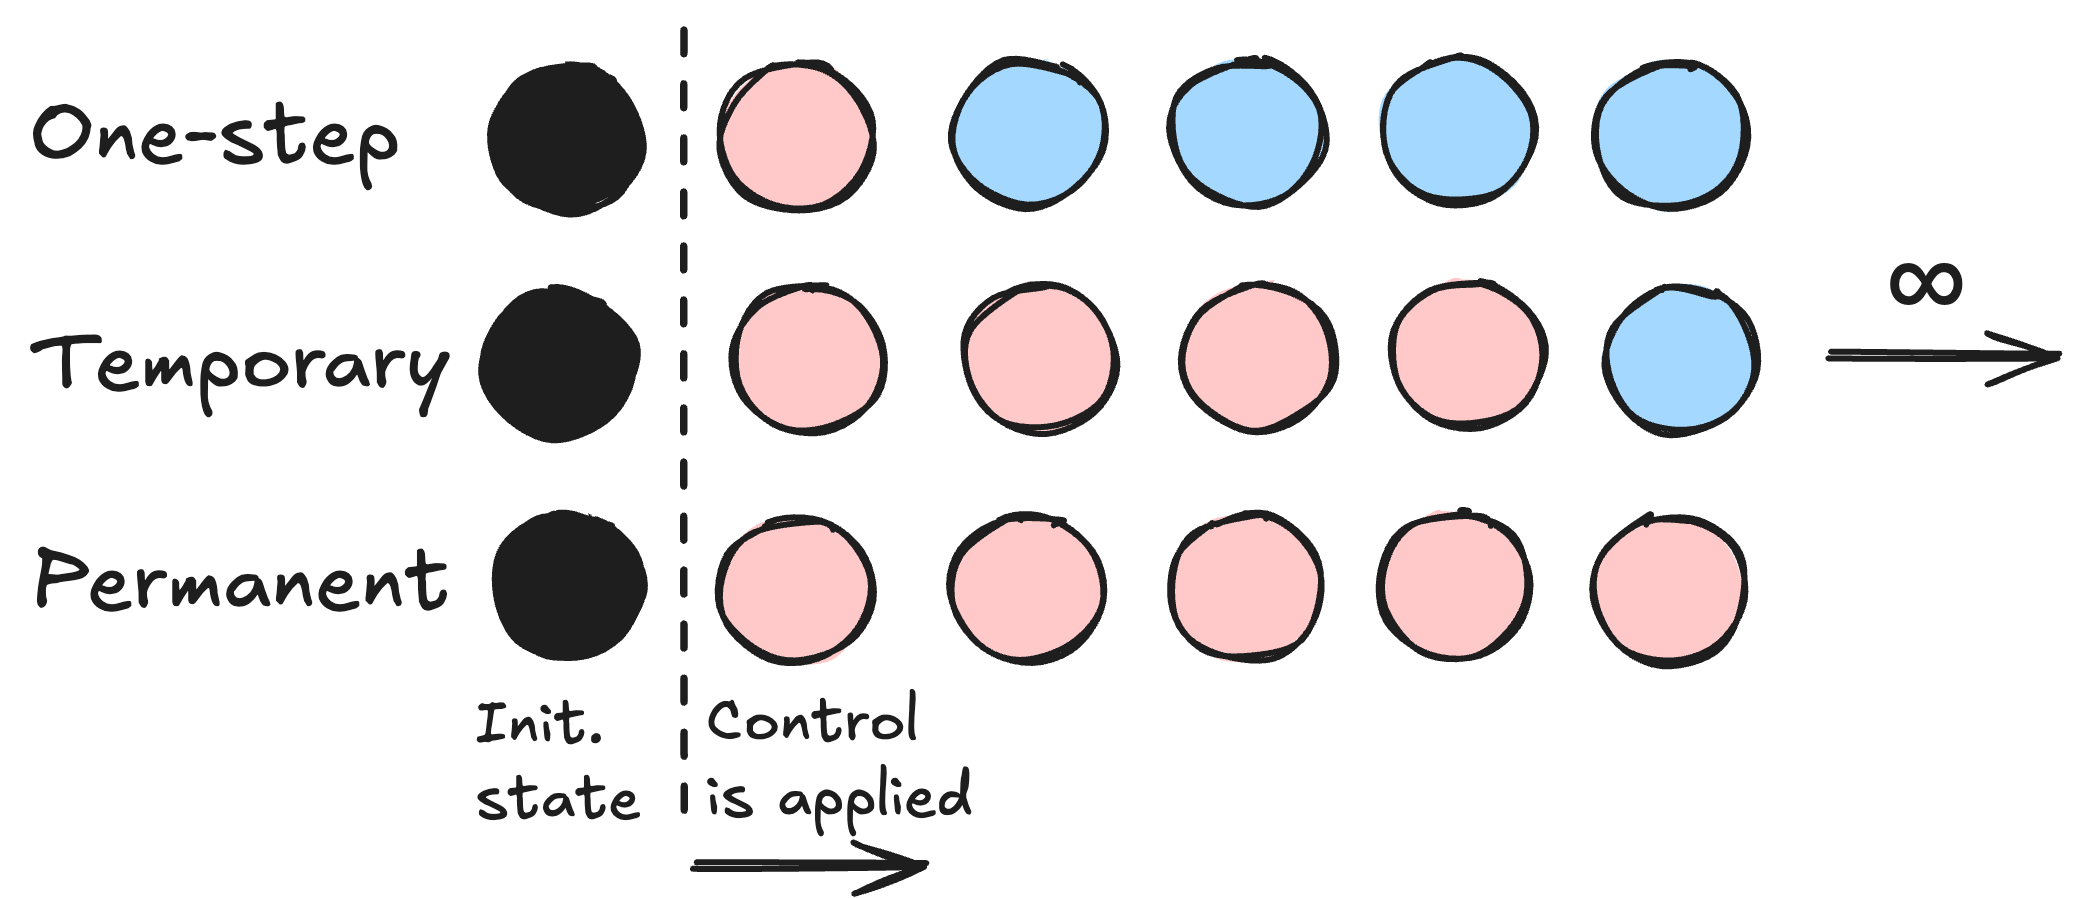
\includegraphics[width=0.8\textwidth]{Figures/otpc.png}
    \caption{
        \textbf{Difference between one-step, temporary and permanent control.} The black markers represent initial states. Red markers represent states which were reached during the time while BN was perturbed and finally, blue markers represent states to which BN transitioned with its natural behavior. The run of BN would continue in the same nature as its last transition.
    }
    \label{fig:otpc}
\end{figure}


\emph{One-step perturbation} (OSP) overrides values of controlled variables once, and then the network is left to evolve in its natural dynamics. Intuitively, the OSP can be viewed as a restriction of the initial states of all BN runs. Technically, the BN run may be at any state before the time step in which the perturbation is applied. Nonetheless, the very next step would bring the network to a state which is part of the OSP. The notion of one-step state perturbation is defined in the following way:

The perturbations applied for multiple time-steps are temporary (TP) and permanent perturbations (PP). As the name suggest, when we use temporary perturbation, there exists a finite amount of time steps after which the perturbation is released, and BN is left to evolve in its natural dynamics. Temporary perturbation applied for only a single time step is equivalent to OSP. 

Finally, the most intrusive perturbations are permanent. This kind of perturbation might be harder to achieve in practice, depending on the specific perturbation context and techniques. Moreover, the permanent perturbation might disrupt the network's original long-term behavior and change the network's attractor landscape; even cause a target attractor to be no longer present in the BN.

To formally define application of perturbations, we differentiate between two types of perturbation applications. The first type is an application to a specific source state, as is the case of source-target control.

\begin{definition}
    \label{def:perturbation_application}
    Given a BN $\bnMath = \{f_1, \ldots, f_n\}$, \emph{application of a perturbation $\perturbation \in \allPerturbations$ to a source state $s \in \bools^n$} is a \emph{forced} state transition (i.e., might not follow the BN standard dynamics), $\pertApply(s, \perturbation) = s \to s'$ such that: 
    $$\pertApply(s_i, \perturbation) = s'_i = \begin{cases}
        s_i & \text{iff } Q_i = \unspecified \\
        Q_i & \text{iff } Q_i \neq \unspecified
    \end{cases}$$
    where $s'$ is the state reached after applying the perturbation.
\end{definition}

After application of a perturbation to a state*\marginpar{*What we call here an application of perturbation (\pertApply) is in some literature called state perturbations and a perturbed BN or runs of perturbed BN are referred to as function perturbations~\cite{Mandon2019PHD}. This is because constants are seen to be an override of variable update function. However, we avoid function perturbation term to avoid confusion with line of work on synchronous Boolean networks where more complex than constant functions are used to perturb networks~\cite{Liu2017}.}, we obtain a state which is \emph{compliant} with the perturbation. This means that the state does not contradict any of the perturbed variables. For example, if we apply perturbation $1\unspecified0$ to state $001$ (contradicting the perturbation at the first variable), we obtain state $101$ which is compliant with the perturbation.

The aforementioned definition is effectively capturing the concept of one-step perturbation for the source-target control. Nonetheless, if we wanted to consider OSP for target or phenotype control, we need to generalize the definition to a whole set of states. To that end, we can adapt the definition above to a set of (all) states and as a result, we obtain a subspace equivalent to the given perturbation as the viable set of initial states.

Another important concept we need to define to understand the application of temporary and permanent perturbations is a \emph{perturbed state transition graph} for a BN:

\begin{definition}
    \label{def:perturbed_stg}
    Given a BN $\bnMath = \{f_1, \ldots, f_n\}$ where $\STG(\bnMath) = (\vertices, \edges)$, \emph{application of a perturbation $\perturbation \in \allPerturbations$ to a Boolean network $\bnMath$} results in a \emph{perturbed Boolean network} $\bnMath_{\perturbation}$ with \emph{perturbed state transition graph} $\STG_{\perturbation}(\bnMath) = (\perturbation, \edges_{\perturbation})$ where vertices are a subspace of the unperturbed state space $\vertices = \bools^n$ given by the perturbation $\perturbation$ and a set of perturbed edges $\edges_{\perturbation} \subseteq \edges$ is given as follows:
    $$
    \edges_{\perturbation} = \{(u, v') \mid (u, v) \in \edges \land u \in Q \land v \in \perturbation\}
    $$
\end{definition}

We can see, that by definition, the perturbed state transition graph is a subgraph of the original state transition graph, containing only the states and transitions that are not violating the perturbation. On the other hand, the perturbed STG might contain different attractors than the original STG. For example trivially, if a BN contains a steady-state attractor, and we apply a perturbation that contradicts some variable of the attractor, the attractor may no longer be present in the perturbed STG. Another example can be seen in \autoref{fig:pert_stg} where due to perturbation the former attractor $1\unspecified\unspecified$ is no longer present and is replaced by the steady-state attractor $110$.

\begin{figure}[bth]
    \centering
    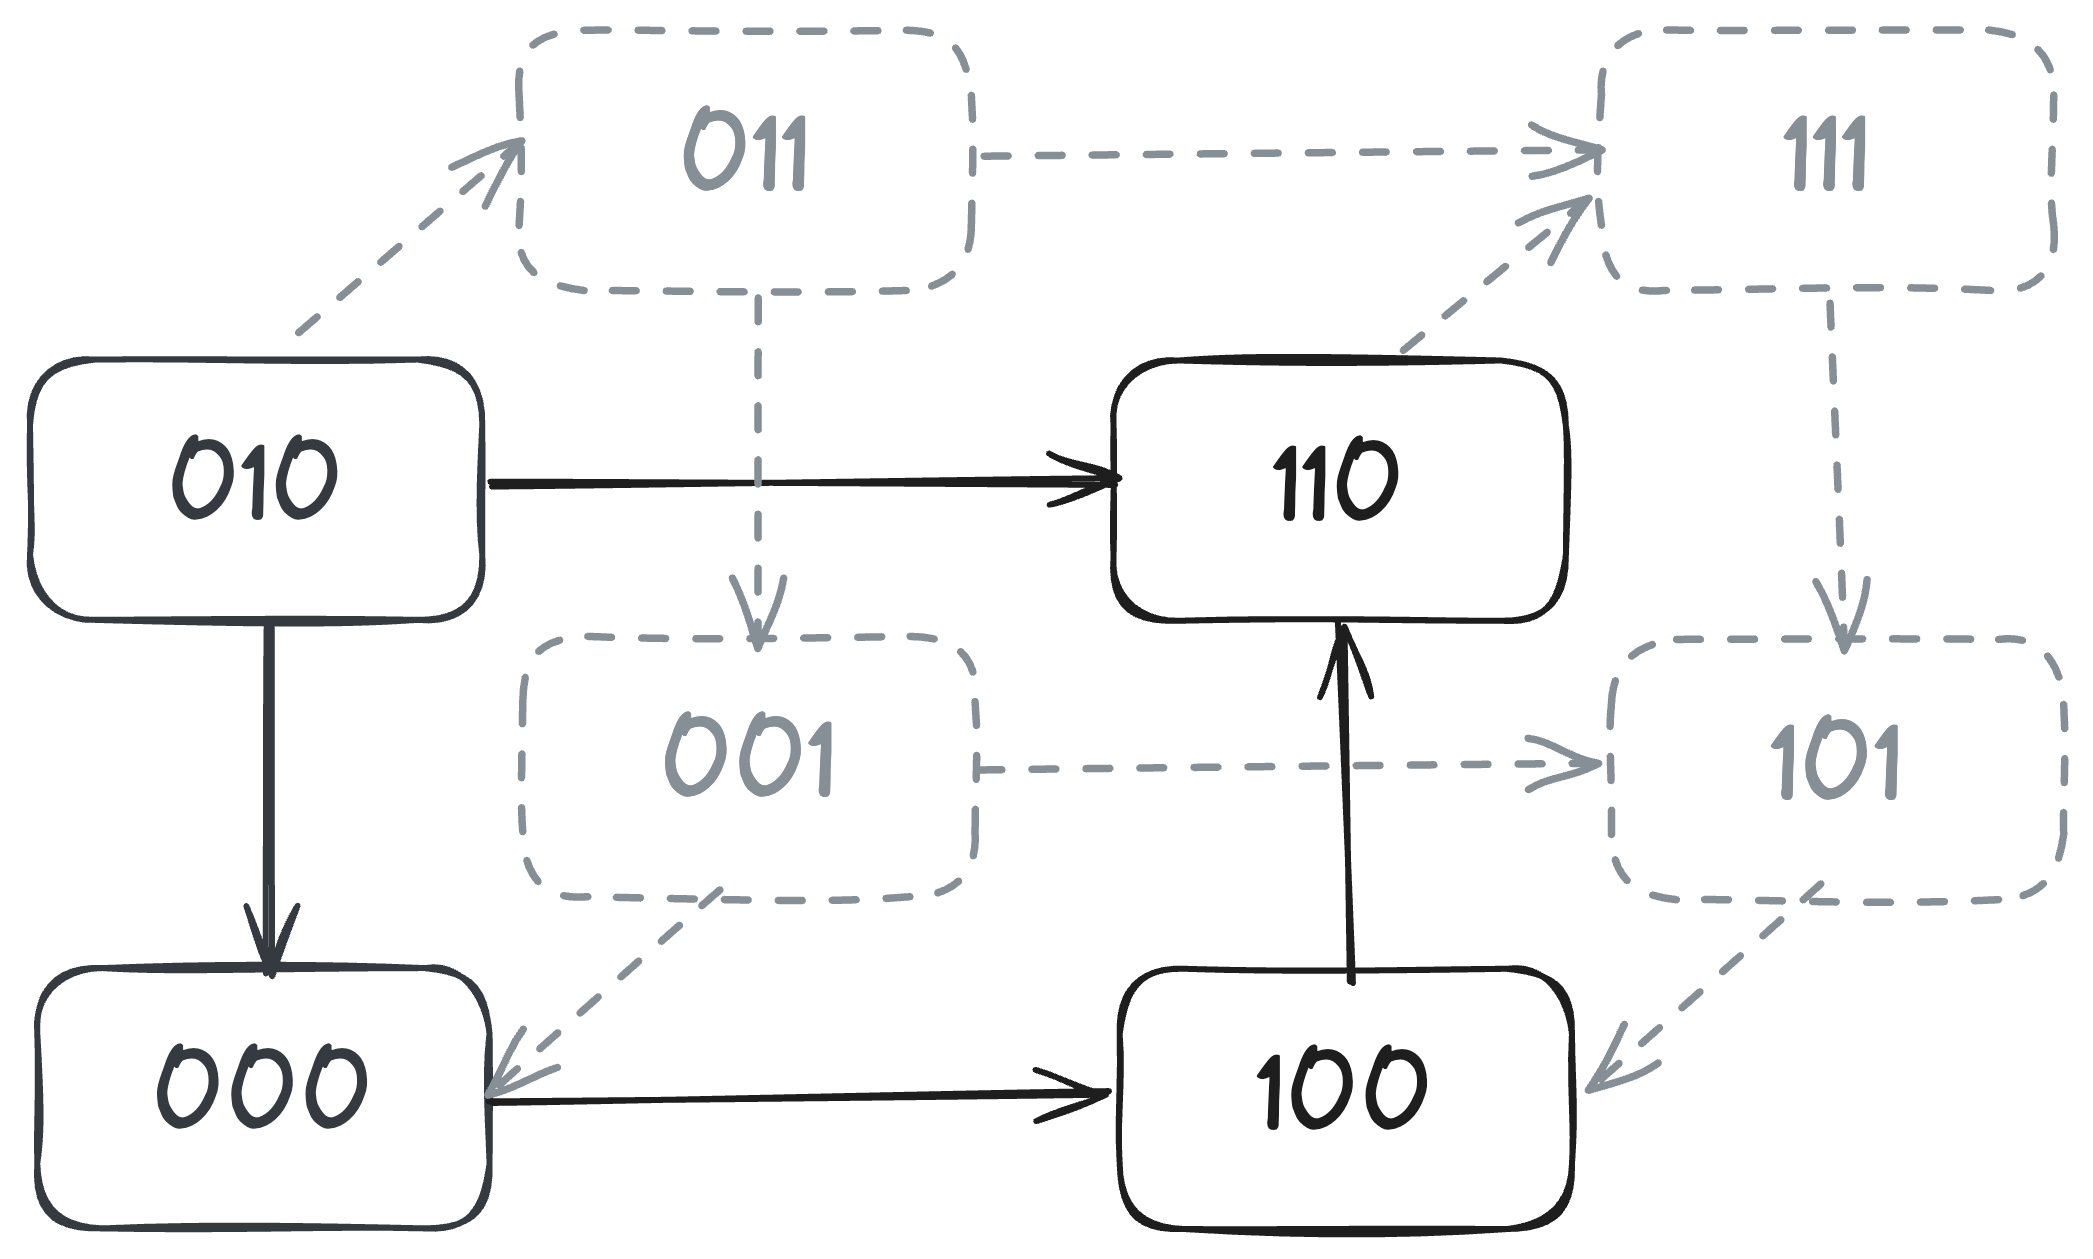
\includegraphics[width=0.45\textwidth]{Figures/perturbed_simple_stg.png}
    \caption{
        \textbf{A perturbed state transition graph of a Boolean network.} The depicted STG is a perturbed version of the STG from \autoref{subfig:stg} under perturbation $\unspecified\unspecified0$. The black solid vertices and edges mark the states and transitions that are preserved in the perturbed STG while the gray dashed vertices and edges represent the states and transitions that have been removed due to not being consistent with the perturbation.}
    \label{fig:pert_stg}
\end{figure}

Now, we can define a perturbed run of a BN:

\begin{definition}
    \label{def:perturbed_run}
    Let us assume a BN $\bnMath = \{f_1, \ldots, f_n\}$, a source states $S \subseteq \bools^n$, a perturbation $\perturbation \in \allPerturbations$, a time period $z \in \Nats_{\infty}$, after which the perturbation is withheld and a natural run $\run \in \STG(\bnMath)$, such that there exists a time-step $t'$ where $\run(t') \in S$. \emph{A perturbed run $\run_{\perturbation}$} is a run which satisfies the following conditions:
    $$
    \run_{\perturbation}(t) = \begin{cases}
        \run(t) & \text{iff } t \leq t' \\
        \pertApply(t, \perturbation) & \text{iff } t = t' + 1 \\
        s'  \text{ s. t. } \run(t-1) = s'' \land (s'', s') \in \edges_{\perturbation} & \text{iff }  t'+z > t > t' + 1 \\
        s'  \text{ s. t. } \run(t-1) = s'' \land (s'', s') \in \edges & \text{iff } t > t'+z
    \end{cases}
    $$
    A set $\allRuns_{\perturbation}(\bnMath, S, z)$ is a collection of all perturbed runs $\run_{\perturbation}$ for a given perturbation $\perturbation$, applied to any state from $S$ with perturbation being withheld after $z$ time-steps.
\end{definition}

 Intuitively, a perturbed run consists of four "stages". First, the run is evolved ``normally" in a given BN. When the BN reaches a state in $S$ (does not need to be the first occurrence of an $s \in S$ in the run), we apply a perturbation to that state. Asz a result, we obtain the nearest state which is compliant with the perturbation. From this state, the BN evolves according to the perturbed STG. If $z$ is not infinite, after $z$ time-steps, the perturbation is withheld, and the BN continues to evolve according to its natural dynamics. 

\begin{example}
An example of a valid perturbed run for a BN from our running example (\autoref{fig:bn_basic}) under perturbation $\unspecified\unspecified0$ applied to a state $101$ and withheld after $z=5$ time-steps is the following:

\begin{itemize}
    \item $t=0 \ldots 2$: The BN evolves naturally, e.g., traverses the states $011 \to 001 \to 101$.
    \item $t=3$: The perturbation $\unspecified\unspecified0$ is applied, resulting in state $100$.
    \item $t=4 \ldots 8$: The BN evolves according to the perturbed STG, reaching state $110$. There are no further viable transitions in the perturbed STG, therefore the BN remains in state $110$.
    \item $t=9$: The perturbation is withheld, and the BN continues to evolve naturally, stabilizing in the attractor $1\unspecified\unspecified$.
\end{itemize}
\end{example}

\begin{table}[htb]
\caption{\textbf{Types of perturbations.} The table summarizes the differences between one-step, temporary, and permanent perturbations when applied to a source-target control, or target types of control (target/full/all-pair/phenotype).}
\begin{tabular}{llll}
 & one-step & temporary & permanent \\
 \hline
source-target & \begin{tabular}[c]{@{}l@{}}$\pertApply(s, \perturbation)$ or\\ $\allRuns_{\perturbation}(\bnMath, \{s\}, 1)$ \end{tabular} & \begin{tabular}[c]{@{}l@{}}$\allRuns_{\perturbation}(\bnMath, \{s\}, z)$\\ s.t. $z \in \Nats$ \end{tabular} & $\allRuns_{\perturbation}(\bnMath, \{s\}, \infty)$\\
\hline
target & \begin{tabular}[c]{@{}l@{}}$\pertApply(\bools^n, \perturbation)$ or\\ $\allRuns_{\perturbation}(\bnMath, \bools^n, 1)$ \end{tabular} & \begin{tabular}[c]{@{}l@{}}$\allRuns_{\perturbation}(\bnMath, \bools^n, z)$\\ s.t. $z \in \Nats$ \end{tabular} & \begin{tabular}[c]{@{}l@{}}$\allRuns_{\perturbation}(\bnMath, \bools^n, \infty)$ or\\ $\bnMath_{\perturbation}$ \end{tabular}
\end{tabular}
\label{tab:perturbation_types}
\end{table}

The \autoref{tab:perturbation_types} summarizes the different types of perturbations and how they can be implemented in the context of different control objectives using the concepts of perturbation application, perturbed STG, and perturbed runs. We can notice, that a one-step control can be seen as a special case of temporary control with time steps sustaining perturbation $z=1$. Moreover, permanent control can be implemented as a perturbed Boolean network.

\begin{figure}[hb!]
    \centering
    \subfloat[Initial perturbation]{
        \label{subfig:ssa_a}
        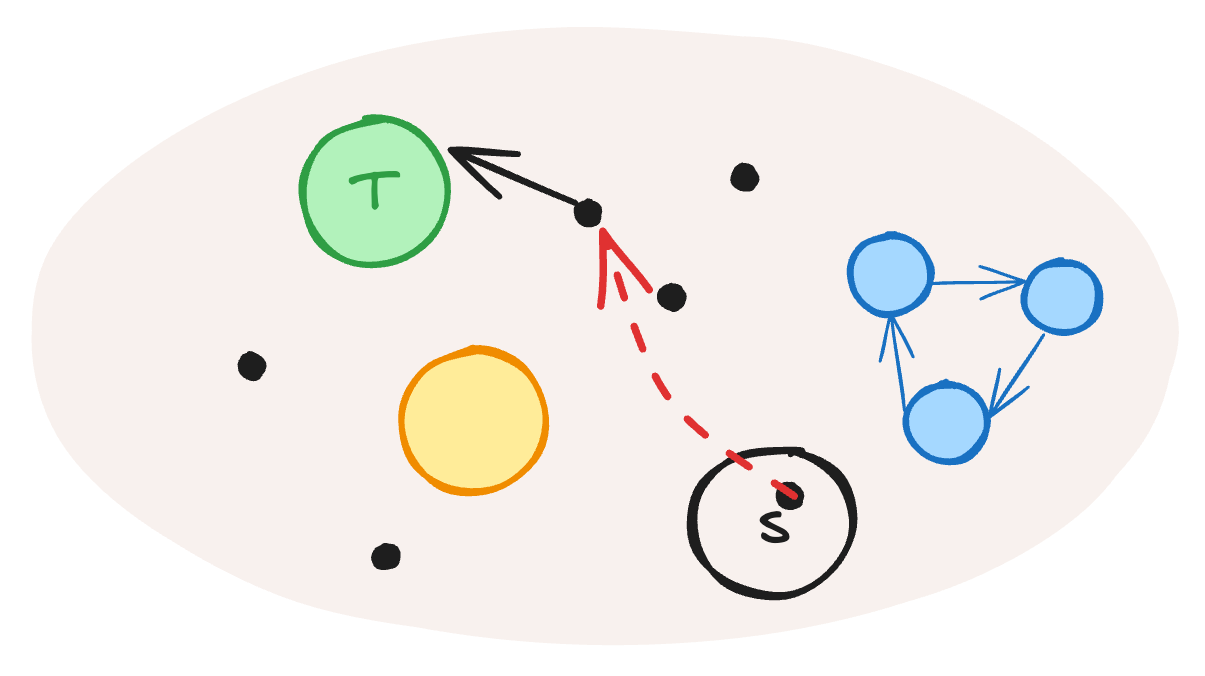
\includegraphics[width=0.4\textwidth,valign=b]{Figures/ssa_a.png}
    }
    \subfloat[Sequential perturbation]{
        \label{subfig:ssa_b}
        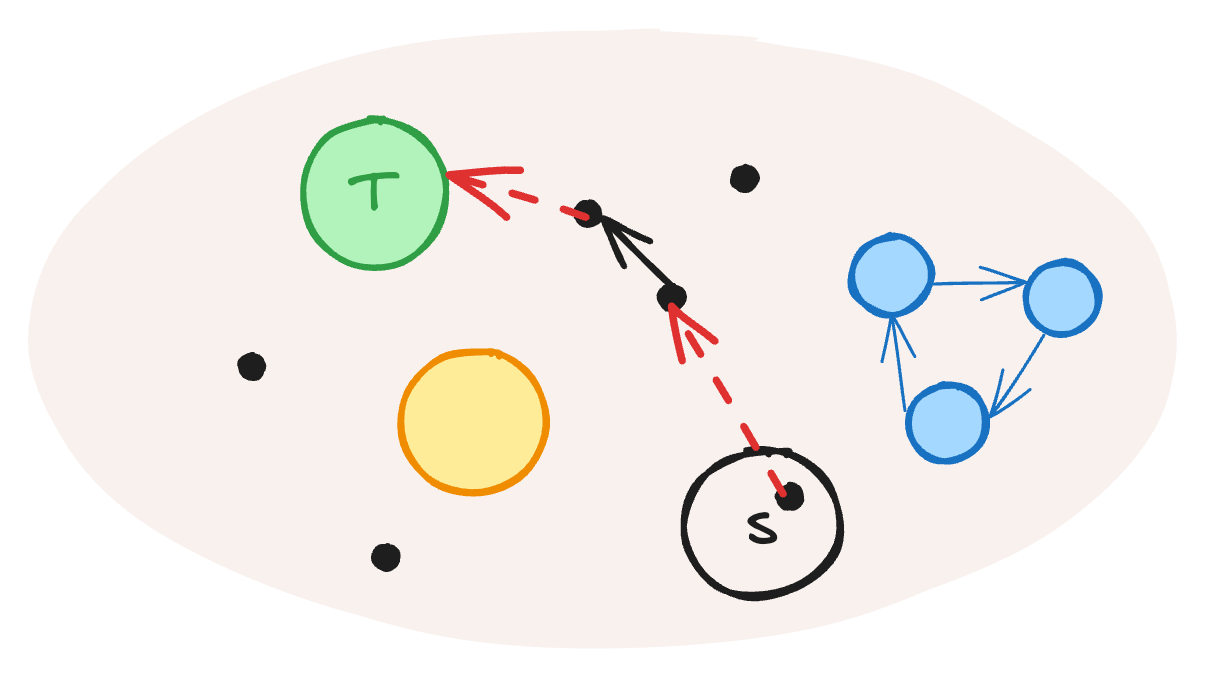
\includegraphics[width=0.4\textwidth,valign=b]{Figures/ssa_b.png}
    }
    \newline
    \subfloat[Sequential attractor-based \newline perturbation]{
        \label{subfig:ssa_c}
        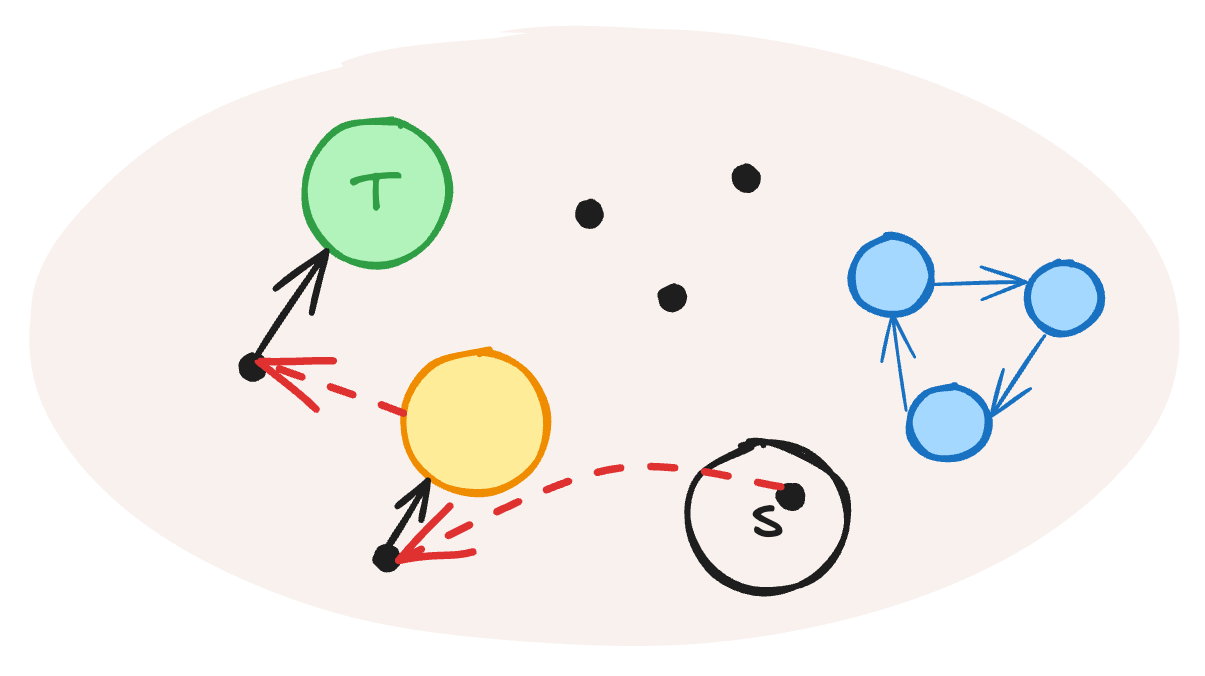
\includegraphics[width=0.4\textwidth,valign=b]{Figures/ssa_c.png}
    }
    \caption{\textbf{Difference between initial, sequential, and sequential attractor-based perturbations.} The figure is only illustrative and does not show precise transitions or perturbations done to the BN. The black points are non-attractor states of BN. The colorful points are attractors, the black arrows are transitions conducted by natural BN dynamics, and the red dashed arrows are transitions done under the effect of perturbations. The initial state is marked as s while the target attractor is the blue one marked with T.} 
    \label{fig:ssa}
\end{figure}

% \intention{Sequential control} 
Some perturbation techniques also consider \emph{when} the perturbations are applied. In \emph{initial} or also referred to as \emph{immediate} control, the perturbations are applied to the given initial state. 

Alternatively, during \emph{sequential} control, (possibly different) perturbations can be applied multiple times at different states. This way, we can potentially control the system using fewer perturbations. However, this approach brings new issues, such as dealing with the non-determinism of the BN (different perturbations may be required for different branches of the non-deterministic network's behavior). 

Moreover, we would need to be able to precisely observe the current state of the BN, which can be very problematic to obtain in practice. These issues can be addressed by using \emph{attractor-based sequential} approach~\cite{Mandon2019CMSB}. Differences between these approaches are depicted in \autoref{fig:ssa}.

In this work, we focus only on the initial control approach, since attractor landscape can be very complex in context of partially specified Boolean networks. On the other hand, the sequential control approach may offer smaller perturbation sizes in certain scenarios that might arise in a future research.

\subsection{Summary}

In summary, the control problems for Boolean networks differ in the following aspects:

\begin{itemize}
\item \emph{What do we want to control; goal}: What is the initial state of the BN? Where we  want to end? Do we want to control only one scenario or multiple scenarios?
\item \emph{What type of perturbations we apply}: We can either perturb states functions of variables.
\item \emph{For how long is perturbation applied}: We can perturb BN only during a single computational step, or we can hold it temporarily, or even forever.
\item \emph{When we apply the perturbations}: Only once at an initial state in contrast with applying control to an arbitrary state and any amount of times.
\end{itemize}

Since in this work, we focus on the control of Boolean networks, in the context of partially specified Boolean networks, we introduce them in the next section.

\section{Partially specified Boolean networks}
\label{s:psbn}
\marginpar{
    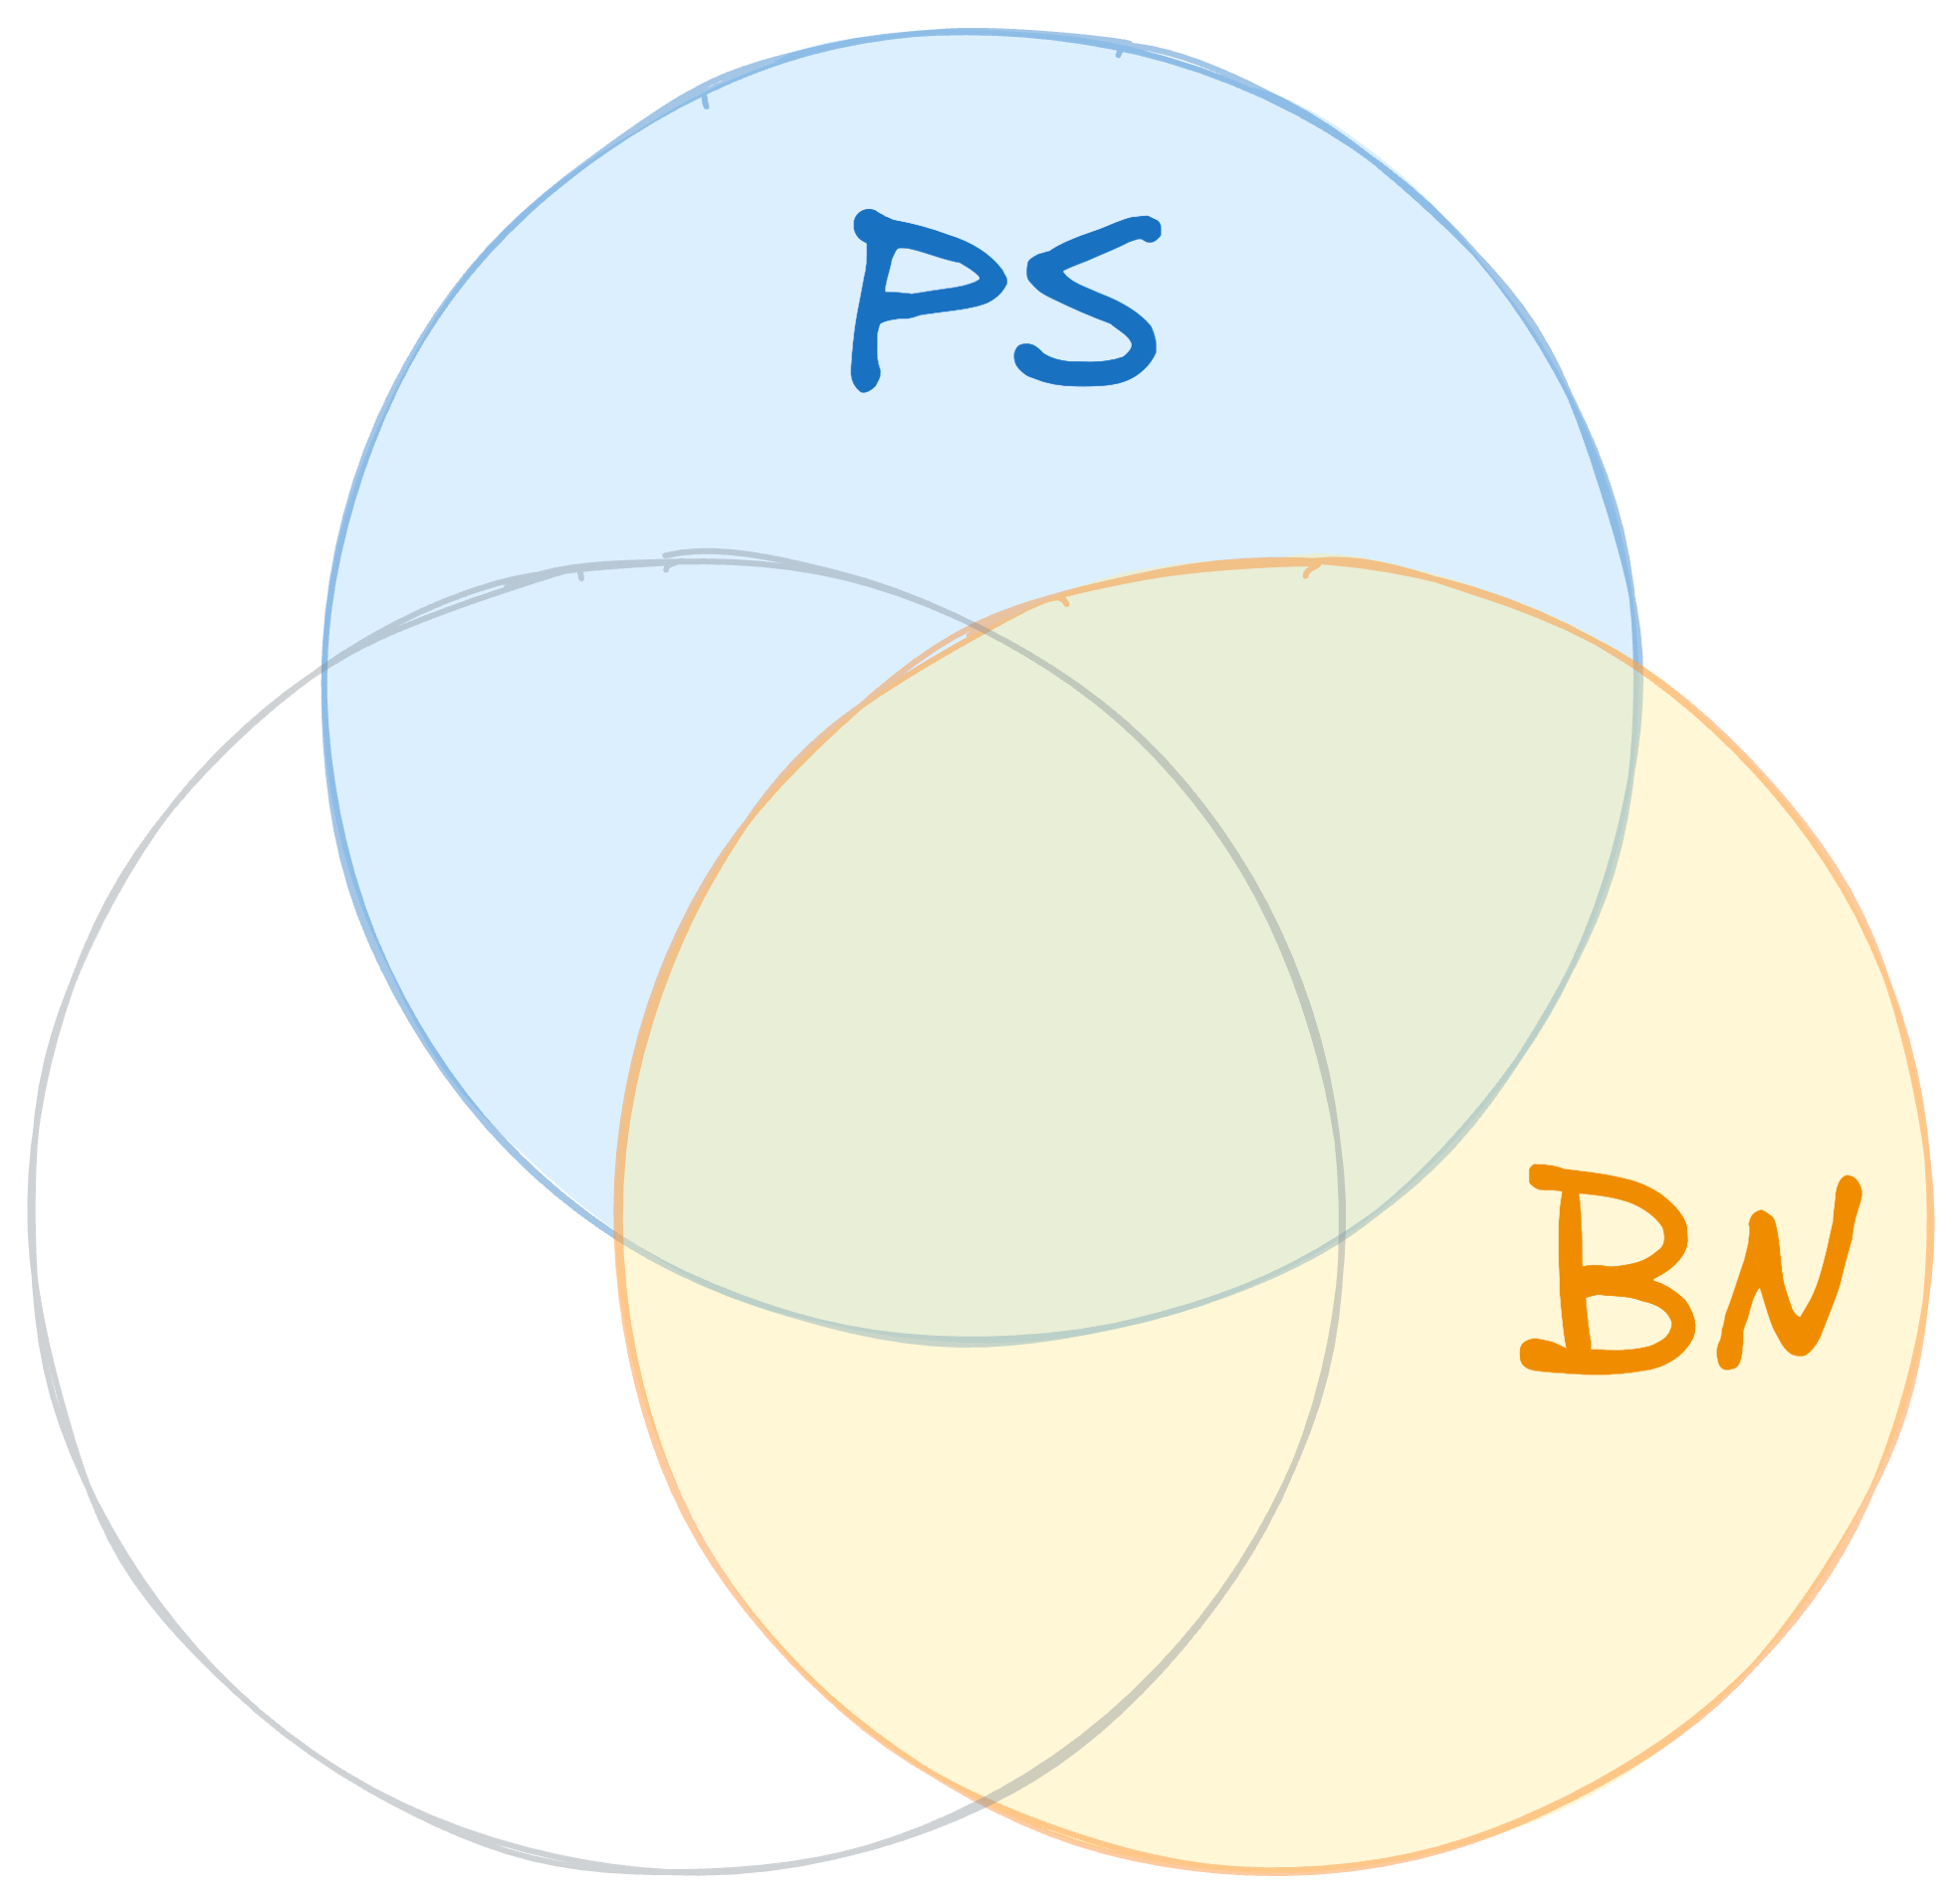
\includegraphics[width=\marginparwidth]{Figures/topics_ps_bns.png}
}


A shortcoming of classical Boolean networks as defined above is that to study network dynamics, all update functions must be fully specified. Moreover, the exact form of the update function might have little impact on observable behavior of the network (i.e., the attractor landscape).

Therefore, it was suggested to observe the dynamics of the Boolean network in context of of Boolean networks ensembles first~\cite{Kauffman2004,Schwab2020}. In this approach, we consider a set of Boolean networks that share some common properties (e.g., the same network structure or the same values of certain variables in their attractors). The goal is to study the dynamics of the whole ensemble instead of a single network. This way, we can obtain more robust results that are not dependent on a specific choice of update functions. 

The ensemble approach described as above, however, has its limitations, as it is not formalized very well and is usually limited to simulations. To address this problem, we consider the notion of \emph{Partially Specified Boolean Networks} (PSBNs)~\cite{Benes2019,benevs2022bdd} (sometimes also termed parametrized Boolean networks or colored Boolean networks). 

In a PSBN, we use \emph{function symbols} as stand-ins for unknown (fixed but arbitrary) parts of the network's unspecified dynamics. Therefore, the dynamics of a variable are either denoted by a standard (fully specified) function or by its function symbol and input arguments.
\begin{definition}
	Let $n$ be the number of variables, and $\allFunSymbols = \{\funSymbol_1,  \dots, \funSymbol_m \}$ a set of \emph{function symbols}. A \emph{partially specified Boolean network} $\pbnMath = \{ \expr_1, \ldots, \expr_n \}$ consists of function symbol expressions given by the following grammar:
	$$
		\expr ::= 0 \mid 1 \mid x \mid \neg \expr \mid \expr \land \expr \mid \expr \lor \expr \mid \funSymbol^{(a)}(\expr, \ldots, \expr) 
	$$
	Here, $x$ ranges over the network variables and $\funSymbol$ over the function symbols of $\allFunSymbols$ (superscript $a \in \mathbb{N}_0$ denotes the arity of $\funSymbol$). Other Boolean operators (e.g. $\Rightarrow$ or $\Leftrightarrow$) can be implemented as syntactic abbreviations using $\lor$, $\land$, and $\neg$.
\end{definition}

In other words, a PSBN is defined using standard Boolean constants ($0$ and $1$), variable state propositions ($x_i$) and Boolean connectives ($\neg$, $\land$, $\lor$), but it can also use function symbols from $\allFunSymbols$ as a way of expressing unknown behavior. This makes it possible to idiomatically describe systems whose dynamics are not fully known (see \autoref{example:psbn}).

\subsection{Interpretations and instances}

To give meaning to a particular $\pbnMath$, we rely on the term \emph{interpretation}. Formally, an interpretation $\interpretation$ is a set of $\{i_1, \ldots, i_m \}$ Boolean functions such that for each $\funSymbol^{(a)} \in \allFunSymbols$, there is a corresponding Boolean function $i^{(a)} \in \interpretation$ of the matching arity $a$. 

Intuitively, an interpretation associates a specific Boolean function to every function symbol. Consequently, we can substitute all symbols $\funSymbol \in \allFunSymbols$ for functions $i \in \interpretation$ in a $\allFunSymbols = \{\funSymbol_1, \ldots, \funSymbol_n\}$ of a $\pbnMath$, and a result we obtain a collection of $n$ fully specified functions. The result is a \emph{Boolean network instance} which we denote as $\pbnMath(\interpretation)$ and which has the same semantics as a standard BN. The set of all possible interpretations of $\allFunSymbols$ is denoted as $\allInterpretations(\allFunSymbols)$ or $\allInterpretations$ for short (i.e., when the context is clear). Some subset of interpretations is then referred to as $\interpretationSet \subseteq \allInterpretations$. 

\subsection[Normalization of PSBN]{Normalization of partially specified Boolean networks}

Function symbols are practical as a human-friendly specification language of unknown network behavior. However, it is not entirely clear how algorithms should represent such functions symbolically, as is our goal in this paper. To alleviate this issue, we note the following: Assuming that all $m$ function symbols in $\allFunSymbols$ have arity zero, possible interpretations $\allInterpretations$ of $\allFunSymbols$ correspond to the vectors $\bools^{m}$. This is because a nullary function symbol is necessarily a constant and can be thus interpreted as a Boolean value. We call such zero arity symbols \emph{zero-arity symbols} (we can also simply write $\funSymbol$ instead of $\allFunSymbols^{(0)}()$ when using such symbols). In some literature, these are also referred to as network inputs~\cite{Kobayashi2011}. 

Given any $\pbnMath$, we can produce a \emph{normalized} $\widehat{\pbnMath}$ that only uses a fresh set of logical nullary function symbols $\widehat{\allFunSymbols}$ instead of general function symbols $\allFunSymbols$, but its interpretations are the same fully specified BNs as for the original $\pbnMath$. To implement this normalization, we use the following expansion rule (here, $\expr_1, \ldots, \expr_a$ are arbitrary Boolean expressions):
\begin{align*}
	\allFunSymbols^{(a)}(\expr_1, \ldots, \expr_a) &\equiv (\expr_1 \Rightarrow \mathcal{F}^{(a-1)}_P(\expr_2, \ldots, \expr_a)) \\
    &\land (\neg \expr_1 \Rightarrow \funSymbol^{(a-1)}_N(\expr_2, \ldots, \expr_a))
\end{align*}

This rule transforms any expression using a function symbol $\funSymbol$ of arity $a$ into an expression using two fresh function symbols of arity $a-1$ ($\funSymbol_P$ and $\funSymbol_N$). Interpretations of the original and the transformed expression result in the same concrete Boolean functions. By recursively applying this rule, we can transform any $\funSymbol^{(a)}$ into $2^a$ nullary function symbols, each corresponding to one row of the truth table of the original $\funSymbol$. Without the loss of generality, we can thus assume that the interpretations of a particular $\pbnMath$ are identified by the members of $\bools^{m}$ for some $m = |\widehat{\allFunSymbols}|$. The set of all interpretations is then exactly equivalent to  $\allInterpretations = \bools^m$. An example of a normalized $\widehat{\pbnMath}$ is given in \autoref{example:psbn}.

We must not forget, that the basis of BNs (and PSBNs) are the regulatory networks as described in \autoref{s:reg_net}. Therefore, if we have a definition of an expression for $x_1$ given as $\expr_1 \equiv \funSymbol(x_1, x_2)$, and we know, that $x_2$ has a down-regulating effect on $x_1$, the functional symbol $\funSymbol$ should \textbf{not} be replaced by a function $x_1 \lor x_2$.

To address this, we will consider the set $\allInterpretations$ to contain only \emph{consistent} interpretations*.\marginpar{*More on the topic of consistent interpretations can be found in a line of work on Boolean networks refinement \cite{Benes2023}.}
 An interpretation $\interpretation$ is consistent with a given regulatory network if for every variable $x_i$ and its corresponding expression $\expr_i$, the function $f_i$ obtained by substituting all function symbols in $\expr_i$ with their corresponding functions from $\interpretation$ respects the regulatory structure of the network. The restrictions on regulations can be found in \autoref{ss:bn_definition}. 

\subsection{Colored state transition graph}
\label{ss:psbn_stg}

\marginpar{*Note, that update schema of PSBNs is different from the probabilistic BNs mentioned in \autoref{ss:updating_schemes}. In particular, the probabilistic semantics use multiple update functions for the same variable within a single run while PSBN considers only a single instance (interpretation) for each run.}
With this knowledge in mind, we can define a \emph{colored} state-transition graph that collectively encodes the behavior of all possible interpretations of a particular $\pbnMath$ using only Boolean values*. In this representation, the interpretations of the normalized $\widehat{\pbnMath}$ (the members of $\bools^m$) each define a potentially different transition relation over the shared state space $\bools^n$:

\begin{definition}
	Let $\widehat{\pbnMath} = \{ \expr_1, \ldots, \expr_n \}$ be a normalized partially specified Boolean network such that $\widehat{\pbnMath}$ admits $m$ nullary function symbols $\allFunSymbols = \{\funSymbol_1, \ldots, \funSymbol_m \}$. The \emph{labelled state-transition graph} $\STG(\widehat{\pbnMath}) = (\vertices, \allInterpretations, \edges)$ is a directed graph where $\vertices = \bools^n$, $\allInterpretations = \bools^m$ and $\edges \subseteq \vertices \times \allInterpretations \times \vertices$ is given as $(u, \interpretation, v) \in \edges \Leftrightarrow (u,v) \in \edges(\STG(\widehat{\pbnMath}(\interpretation)))$. We write a state transition under $\interpretation$ as $u \to_{\interpretation} v$. The set of all interpretations enabling a transition from $u$ to $v$ is denoted as $\interpretationSet(u,v) = \{\interpretation \mid (u, \interpretation, v) \in \edges\}$.
\end{definition}

In other words, the labelled state-transition graph is a unifying structure that incorporates the STG of all instances of $\pbnMath$: A transition from a state $u$ to state $v$ is enabled for an interpretation $\interpretation$ if the same transition appears in the STG of $\pbnMath(\interpretation)$. Similarly, we consider \PBN{} runs in the context of a specific interpretation $\interpretation$ (or instance) denoted as $\allRuns_\interpretation$. An example of an STG of a \PBN{} instance is depicted in \autoref{fig:psbn}. We further explore the usefulness of labelled STGs in \textcolor{red}{Section REF}, where we show how these can be efficiently manipulated symbolically.

\begin{example}
	\label{example:psbn}
	Consider a PSBN $\pbnMath$ with $\allFunSymbols = \{ \funSymbol^{(2)}\}$ and given by three expressions: 
    \begin{align*}
    \expr_1 &\equiv \funSymbol(x_1, x_2) \\
    \expr_2 &\equiv x_1 \land x_3 \\
    \expr_3 &\equiv x_1 \lor \neg x_3
    \end{align*}
    After normalization, we have $\widehat{\allFunSymbols} = \{ \funSymbol_{00}, \funSymbol_{01}, \funSymbol_{10}, \funSymbol_{11} \}$ and expressions:
    \begin{align*}
        \widehat{\expr}_1 &\equiv ((\neg x_1 \land \neg x_2) \Rightarrow \funSymbol_{00}) \\
        &\land ((\neg x_1 \land x_2) \Rightarrow \funSymbol_{01}) \\
        &\land ((x_1 \land \neg x_2) \Rightarrow \funSymbol_{10}) \\
        &\land ((x_1 \land x_2) \Rightarrow \funSymbol_{11}) \\
        \widehat{\expr}_2 &\equiv x_1 \land x_3 \\
        \widehat{\expr}_3 &\equiv x_1 \lor \neg x_3
    \end{align*}
\end{example}


\begin{figure}[htp]
    \centering
    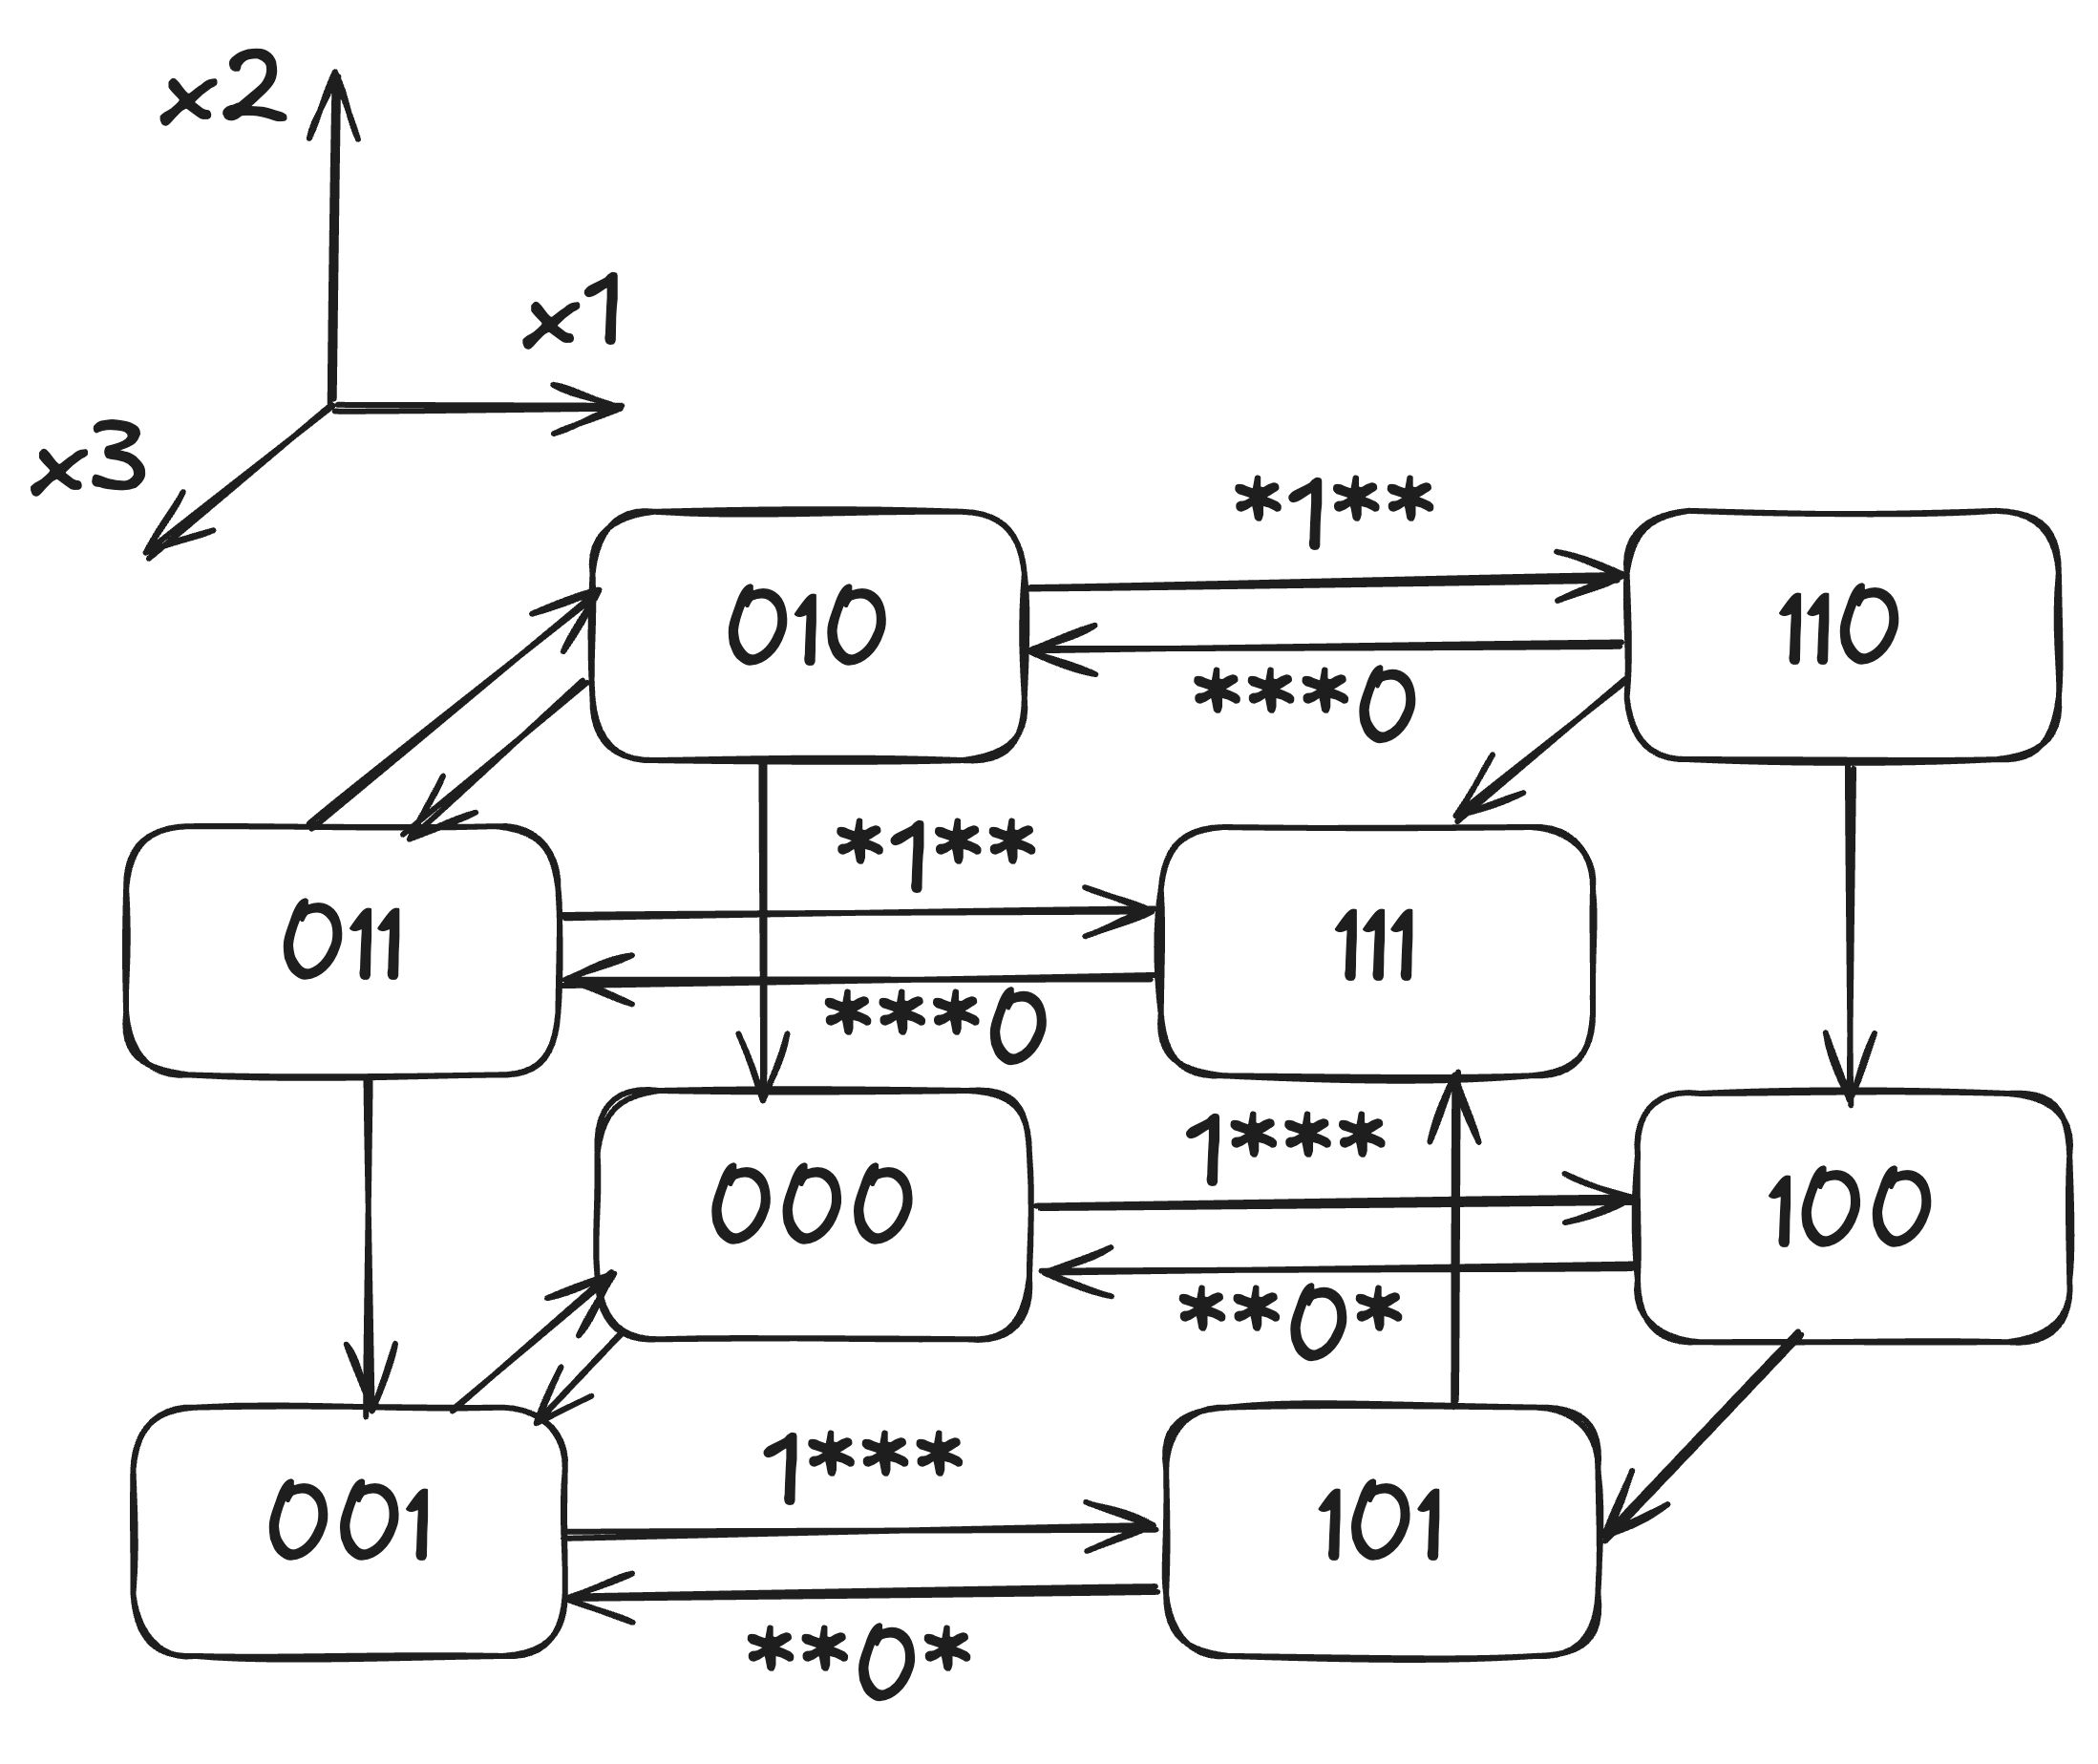
\includegraphics[width=0.5\textwidth]{Figures/psbn_state_space.png}
    \caption{\textbf{State-transition graph of a PSBN.} Figure shows the state-transition graph of a PSBN from \autoref{example:psbn}. The labels of edges represent all interpretations for which the edge is admissible. For brevity, edges admissible in all instances are drawn without a label while edges admissible for no instance are not depicted in the figure at all.}
    \label{fig:psbn}
\end{figure}


Given the notions of labelled STG and a PSBN instance, we can transfer the state space structures previously introduced for BNs to the PSBN setting. We will not focus on the control and perturbation notions, since they are part of the contribution of the thesis and are described in \autoref{chapter:source_target_control} and \autoref{chapter:phenotype_control_psbn}.

The notions which are independent transitions such as character, trait and phenotype do not depend on the actual dynamics of the network (only on its variables) are identical for BNs and PSBNs.

Definitions of trap set, attractor, attractor's weak and strong basins for fully specified BNs are lifted to PSBNs per individual instances (interpretations). For example, we write that a set $\attractor \subseteq \vertices$ is an attractor for an instance $\pbnMath(\interpretation)$ (i.e. there are no attractors of $\pbnMath$, only attractors of its instance). 

\subsection[Well-known problems on PSBNs]{Well-known problems on partially specified Boolean networks}

Now that we have defined PSBNs, we can also consider well-known problems solved for this type of models, in order to understand the challenges they present and give us a better understanding of the tools we can use to solve the control problems. Or vice versa, we can also consider how the control problems can be used to solve the well-known problems on PSBNs.

\subsubsection{Attractor search}

Attractor search in PSBNs involves identifying sets of states (attractors) that the system tends to evolve towards, regardless of the initial state. This is crucial for understanding the long-term behavior of the networks. As opposed to fully specified BNs, PSBNs can have a significantly larger number of attractors due to the uncertainty in their dynamics. Moreover, the attractors can differ across instances, leading to a more complex attractor landscape.

For PSBNs, usually the approaches from fully specified BNs are applied, but they are either highly parallelized or adjusted to work with the labelled STG. For example, one can use symbolic methods to represent and manipulate the state space efficiently, allowing for the exploration of multiple interpretations simultaneously~\cite{benevs2022bdd,Pauleve2023b}.

In context of control, attractor search is often a preliminary step to identify potential target states or behaviors that we want to achieve through control interventions. It also serves as a good last step to verify if the control objectives have been met.

\subsubsection{Bifurcation}

As described before, bifurcation analysis studies how changes in parameters (in the case of PSBNs, interpretations) can lead to qualitative changes in the system's dynamics. In PSBNs, this involves examining how different interpretations affect the attractor landscape and identifying critical interpretations that lead to significant changes in behavior~\cite{Benes2022, Pastva2022}.

This problem is particularly relevant in biological contexts, where certain gene regulatory networks may exhibit different behaviors under varying conditions or mutations. Bifurcation analysis can help identify these critical points and understand the robustness of the network's behavior.

In context of control of PSBNs, bifurcation analysis again can be used as an aid for attractor search and deciding suitable target attractors. 

\subsubsection{Model checking}

Model checking in PSBNs involves verifying whether certain properties or specifications hold across all possible interpretations of the network. This is particularly challenging due to the combinatorial explosion of possible interpretations, but it is essential for ensuring that the network behaves as expected under various conditions~\cite{Benes2023}. 

Model checking can be used to verify safety properties (e.g., certain undesirable states are never reached), liveness properties (e.g., certain desirable states are eventually reached), and other temporal properties of interest. In the context of control, model checking can be used to verify whether the control strategies employed lead to the desired outcomes across all interpretations of the PSBN.

\subsubsection{Model refinement}

All the methods above are also often used for the grand objective of \emph{model refinement}, which aims to reduce the uncertainty in a PSBN by eliminating interpretations that are inconsistent with observed data or desired properties. This process helps in narrowing down the set of possible network behaviors, making the model more precise and reliable~\cite{Benes2023}. Such a model is more likely to yield accurate predictions and insights into the underlying biological processes.

In the context of control, model refinement can help in identifying more effective control strategies by omitting spurious network behaviors. But also vice versa, as we describe in \autoref{chapter:applications}, we suggest control to be used as another tool for model refinement.

\section{Summary}

In this chapter, we have introduced the necessary background for understanding the control of Boolean networks. We started by defining regulatory networks, and Boolean networks and their dynamics, including the concept of attractors and basins of attraction.

We then discussed various control objectives, types of perturbations that can be applied to control the network, including one-step, temporary, and permanent perturbations, as well as their temporal properties.

Finally, we introduced partially specified Boolean networks, which allow for the representation of uncertainty in network dynamics, and discussed their normalization and the concept of a colored state transition graph. 

This foundational knowledge sets the stage for the subsequent chapters, where we will delve into specific control strategies and algorithms for both fully specified (in terms of state of the art) and partially specified Boolean networks (in terms of contribution of this thesis).